\documentclass[twoside]{book}

% Packages required by doxygen
\usepackage{fixltx2e}
\usepackage{calc}
\usepackage{doxygen}
\usepackage[export]{adjustbox} % also loads graphicx
\usepackage{graphicx}
\usepackage[utf8]{inputenc}
\usepackage{makeidx}
\usepackage{multicol}
\usepackage{multirow}
\PassOptionsToPackage{warn}{textcomp}
\usepackage{textcomp}
\usepackage[nointegrals]{wasysym}
\usepackage[table]{xcolor}

% Font selection
\usepackage[T1]{fontenc}
\usepackage[scaled=.90]{helvet}
\usepackage{courier}
\usepackage{amssymb}
\usepackage{sectsty}
\renewcommand{\familydefault}{\sfdefault}
\allsectionsfont{%
  \fontseries{bc}\selectfont%
  \color{darkgray}%
}
\renewcommand{\DoxyLabelFont}{%
  \fontseries{bc}\selectfont%
  \color{darkgray}%
}
\newcommand{\+}{\discretionary{\mbox{\scriptsize$\hookleftarrow$}}{}{}}

% Page & text layout
\usepackage{geometry}
\geometry{%
  a4paper,%
  top=2.5cm,%
  bottom=2.5cm,%
  left=2.5cm,%
  right=2.5cm%
}
\tolerance=750
\hfuzz=15pt
\hbadness=750
\setlength{\emergencystretch}{15pt}
\setlength{\parindent}{0cm}
\setlength{\parskip}{3ex plus 2ex minus 2ex}
\makeatletter
\renewcommand{\paragraph}{%
  \@startsection{paragraph}{4}{0ex}{-1.0ex}{1.0ex}{%
    \normalfont\normalsize\bfseries\SS@parafont%
  }%
}
\renewcommand{\subparagraph}{%
  \@startsection{subparagraph}{5}{0ex}{-1.0ex}{1.0ex}{%
    \normalfont\normalsize\bfseries\SS@subparafont%
  }%
}
\makeatother

% Headers & footers
\usepackage{fancyhdr}
\pagestyle{fancyplain}
\fancyhead[LE]{\fancyplain{}{\bfseries\thepage}}
\fancyhead[CE]{\fancyplain{}{}}
\fancyhead[RE]{\fancyplain{}{\bfseries\leftmark}}
\fancyhead[LO]{\fancyplain{}{\bfseries\rightmark}}
\fancyhead[CO]{\fancyplain{}{}}
\fancyhead[RO]{\fancyplain{}{\bfseries\thepage}}
\fancyfoot[LE]{\fancyplain{}{}}
\fancyfoot[CE]{\fancyplain{}{}}
\fancyfoot[RE]{\fancyplain{}{\bfseries\scriptsize Generated by Doxygen }}
\fancyfoot[LO]{\fancyplain{}{\bfseries\scriptsize Generated by Doxygen }}
\fancyfoot[CO]{\fancyplain{}{}}
\fancyfoot[RO]{\fancyplain{}{}}
\renewcommand{\footrulewidth}{0.4pt}
\renewcommand{\chaptermark}[1]{%
  \markboth{#1}{}%
}
\renewcommand{\sectionmark}[1]{%
  \markright{\thesection\ #1}%
}

% Indices & bibliography
\usepackage{natbib}
\usepackage[titles]{tocloft}
\setcounter{tocdepth}{3}
\setcounter{secnumdepth}{5}
\makeindex

% Hyperlinks (required, but should be loaded last)
\usepackage{ifpdf}
\ifpdf
  \usepackage[pdftex,pagebackref=true]{hyperref}
\else
  \usepackage[ps2pdf,pagebackref=true]{hyperref}
\fi
\hypersetup{%
  colorlinks=true,%
  linkcolor=blue,%
  citecolor=blue,%
  unicode%
}

% Custom commands
\newcommand{\clearemptydoublepage}{%
  \newpage{\pagestyle{empty}\cleardoublepage}%
}

\usepackage{caption}
\captionsetup{labelsep=space,justification=centering,font={bf},singlelinecheck=off,skip=4pt,position=top}

%===== C O N T E N T S =====

\begin{document}

% Titlepage & ToC
\hypersetup{pageanchor=false,
             bookmarksnumbered=true,
             pdfencoding=unicode
            }
\pagenumbering{alph}
\begin{titlepage}
\vspace*{7cm}
\begin{center}%
{\Large Guillermo Hernández González Max Disperity }\\
\vspace*{1cm}
{\large Generated by Doxygen 1.8.13}\\
\end{center}
\end{titlepage}
\clearemptydoublepage
\pagenumbering{roman}
\tableofcontents
\clearemptydoublepage
\pagenumbering{arabic}
\hypersetup{pageanchor=true}

%--- Begin generated contents ---
\chapter{Hierarchical Index}
\section{Class Hierarchy}
This inheritance list is sorted roughly, but not completely, alphabetically\+:\begin{DoxyCompactList}
\item \contentsline{section}{Algorithm}{\pageref{classAlgorithm}}{}
\begin{DoxyCompactList}
\item \contentsline{section}{greedy\+Algorithm}{\pageref{classgreedyAlgorithm}}{}
\item \contentsline{section}{local\+Search}{\pageref{classlocalSearch}}{}
\item \contentsline{section}{second\+Greedy\+Algorithm}{\pageref{classsecondGreedyAlgorithm}}{}
\end{DoxyCompactList}
\item \contentsline{section}{Matriz}{\pageref{classMatriz}}{}
\end{DoxyCompactList}

\chapter{Class Index}
\section{Class List}
Here are the classes, structs, unions and interfaces with brief descriptions\+:\begin{DoxyCompactList}
\item\contentsline{section}{\hyperlink{classAlgorithm}{Algorithm} \\*Virtual algorithm class used to solve the maxmean problem }{\pageref{classAlgorithm}}{}
\item\contentsline{section}{\hyperlink{classgreedyAlgorithm}{greedy\+Algorithm} \\*Implementation of the greedy algorithm to solve Maximum diversity problem }{\pageref{classgreedyAlgorithm}}{}
\item\contentsline{section}{\hyperlink{classlocalSearch}{local\+Search} \\*Implementation of the Local Search algorithm }{\pageref{classlocalSearch}}{}
\item\contentsline{section}{\hyperlink{classMatriz}{Matriz} \\*Matrix containing all the distances between nodes }{\pageref{classMatriz}}{}
\item\contentsline{section}{\hyperlink{classsecondGreedyAlgorithm}{second\+Greedy\+Algorithm} \\*Another implementation of the greedy algorithm to solve Maximum diversity problem }{\pageref{classsecondGreedyAlgorithm}}{}
\end{DoxyCompactList}

\chapter{File Index}
\section{File List}
Here is a list of all documented files with brief descriptions\+:\begin{DoxyCompactList}
\item\contentsline{section}{include/\hyperlink{2ndGreedyAlgorithm_8hpp}{2nd\+Greedy\+Algorithm.\+hpp} \\*Fichero que contiene la implementación del algoritmo greedy de forma destructiva }{\pageref{2ndGreedyAlgorithm_8hpp}}{}
\item\contentsline{section}{include/\hyperlink{algorithm_8hpp}{algorithm.\+hpp} \\*Fichero que contiene la clase \hyperlink{classAlgorithm}{Algorithm} que servirá como clase base para la implementación de los otros algoritmos }{\pageref{algorithm_8hpp}}{}
\item\contentsline{section}{include/\hyperlink{greedyAlgorithm_8hpp}{greedy\+Algorithm.\+hpp} \\*Fichero que contiene la implementación del algoritmo greedy de forma constructiva }{\pageref{greedyAlgorithm_8hpp}}{}
\item\contentsline{section}{include/\hyperlink{localSearch_8hpp}{local\+Search.\+hpp} \\*Fichero que contiene la implementación de la búsqueda local }{\pageref{localSearch_8hpp}}{}
\item\contentsline{section}{include/{\bfseries Matrix.\+hpp} }{\pageref{Matrix_8hpp}}{}
\end{DoxyCompactList}

\chapter{Class Documentation}
\hypertarget{classAlgorithm}{}\section{Algorithm Class Reference}
\label{classAlgorithm}\index{Algorithm@{Algorithm}}


virtual algorithm class used to solve the maxmean problem  




{\ttfamily \#include $<$algorithm.\+hpp$>$}



Inheritance diagram for Algorithm\+:
\nopagebreak
\begin{figure}[H]
\begin{center}
\leavevmode
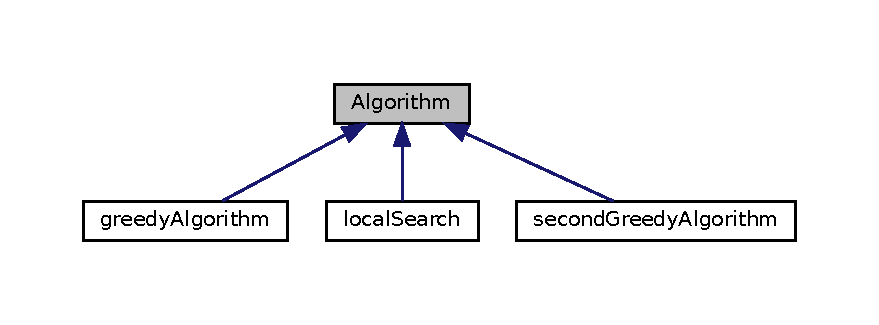
\includegraphics[width=350pt]{classAlgorithm__inherit__graph}
\end{center}
\end{figure}


Collaboration diagram for Algorithm\+:
\nopagebreak
\begin{figure}[H]
\begin{center}
\leavevmode
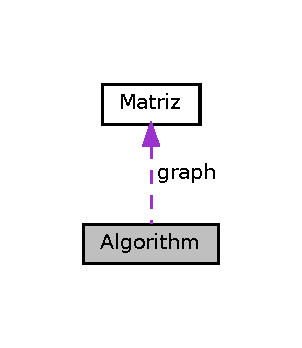
\includegraphics[width=145pt]{classAlgorithm__coll__graph}
\end{center}
\end{figure}
\subsection*{Public Member Functions}
\begin{DoxyCompactItemize}
\item 
\hyperlink{classAlgorithm_a3c199c8528aae86f06ac515d5102fa09}{Algorithm} (std\+::string filename, int sol)
\begin{DoxyCompactList}\small\item\em Construct a new \hyperlink{classAlgorithm}{Algorithm} object. \end{DoxyCompactList}\item 
virtual std\+::vector$<$ int $>$ \hyperlink{classAlgorithm_af6ea9eb9a6dbd41896e3fd7dabac096b}{execute} ()=0
\begin{DoxyCompactList}\small\item\em Method that executes the algorithm. \end{DoxyCompactList}\end{DoxyCompactItemize}
\subsection*{Protected Attributes}
\begin{DoxyCompactItemize}
\item 
\mbox{\Hypertarget{classAlgorithm_ac738351f4331aee2fb965f689b7be273}\label{classAlgorithm_ac738351f4331aee2fb965f689b7be273}} 
\hyperlink{classMatriz}{Matriz} {\bfseries graph}
\item 
\mbox{\Hypertarget{classAlgorithm_a605f2288613c21d986485ec0feef6851}\label{classAlgorithm_a605f2288613c21d986485ec0feef6851}} 
int {\bfseries solution\+Size}
\end{DoxyCompactItemize}


\subsection{Detailed Description}
virtual algorithm class used to solve the maxmean problem 

\subsection{Constructor \& Destructor Documentation}
\mbox{\Hypertarget{classAlgorithm_a3c199c8528aae86f06ac515d5102fa09}\label{classAlgorithm_a3c199c8528aae86f06ac515d5102fa09}} 
\index{Algorithm@{Algorithm}!Algorithm@{Algorithm}}
\index{Algorithm@{Algorithm}!Algorithm@{Algorithm}}
\subsubsection{\texorpdfstring{Algorithm()}{Algorithm()}}
{\footnotesize\ttfamily Algorithm\+::\+Algorithm (\begin{DoxyParamCaption}\item[{std\+::string}]{filename,  }\item[{int}]{sol }\end{DoxyParamCaption})\hspace{0.3cm}{\ttfamily [inline]}}



Construct a new \hyperlink{classAlgorithm}{Algorithm} object. 


\begin{DoxyParams}{Parameters}
{\em filename} & \\
\hline
\end{DoxyParams}

\begin{DoxyCode}
36 : graph(filename), solutionSize(sol)\{\};
\end{DoxyCode}
Here is the call graph for this function\+:
\nopagebreak
\begin{figure}[H]
\begin{center}
\leavevmode
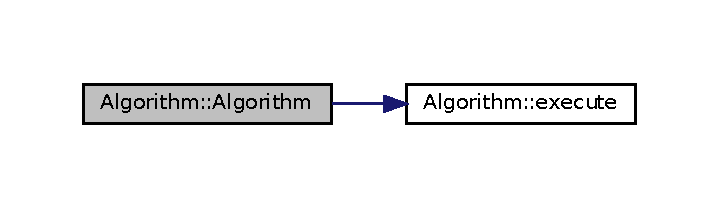
\includegraphics[width=345pt]{classAlgorithm_a3c199c8528aae86f06ac515d5102fa09_cgraph}
\end{center}
\end{figure}


\subsection{Member Function Documentation}
\mbox{\Hypertarget{classAlgorithm_af6ea9eb9a6dbd41896e3fd7dabac096b}\label{classAlgorithm_af6ea9eb9a6dbd41896e3fd7dabac096b}} 
\index{Algorithm@{Algorithm}!execute@{execute}}
\index{execute@{execute}!Algorithm@{Algorithm}}
\subsubsection{\texorpdfstring{execute()}{execute()}}
{\footnotesize\ttfamily virtual std\+::vector$<$int$>$ Algorithm\+::execute (\begin{DoxyParamCaption}{ }\end{DoxyParamCaption})\hspace{0.3cm}{\ttfamily [pure virtual]}}



Method that executes the algorithm. 

\begin{DoxyReturn}{Returns}
std\+::vector$<$int$>$ 
\end{DoxyReturn}


Implemented in \hyperlink{classsecondGreedyAlgorithm_a119a730116003d00438179ccf4e2cafd}{second\+Greedy\+Algorithm}, \hyperlink{classgreedyAlgorithm_a37c81600b24a32ae25b6f0eeab643a7a}{greedy\+Algorithm}, and \hyperlink{classlocalSearch_a0ac1d7bf221f1ab7af92f1a91017cf02}{local\+Search}.

Here is the caller graph for this function\+:
\nopagebreak
\begin{figure}[H]
\begin{center}
\leavevmode
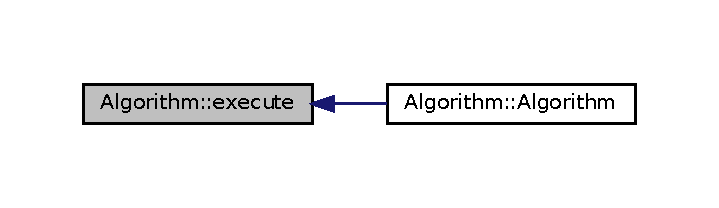
\includegraphics[width=345pt]{classAlgorithm_af6ea9eb9a6dbd41896e3fd7dabac096b_icgraph}
\end{center}
\end{figure}


The documentation for this class was generated from the following file\+:\begin{DoxyCompactItemize}
\item 
include/\hyperlink{algorithm_8hpp}{algorithm.\+hpp}\end{DoxyCompactItemize}

\hypertarget{classgreedyAlgorithm}{}\section{greedy\+Algorithm Class Reference}
\label{classgreedyAlgorithm}\index{greedy\+Algorithm@{greedy\+Algorithm}}


Implementation of the greedy algorithm to solve Maximum diversity problem.  




{\ttfamily \#include $<$greedy\+Algorithm.\+hpp$>$}



Inheritance diagram for greedy\+Algorithm\+:
\nopagebreak
\begin{figure}[H]
\begin{center}
\leavevmode
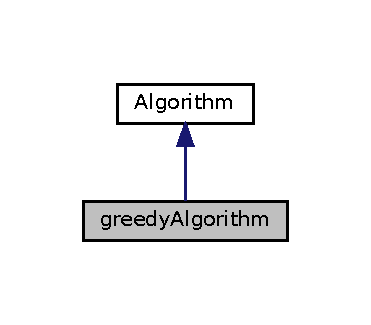
\includegraphics[width=178pt]{classgreedyAlgorithm__inherit__graph}
\end{center}
\end{figure}


Collaboration diagram for greedy\+Algorithm\+:
\nopagebreak
\begin{figure}[H]
\begin{center}
\leavevmode
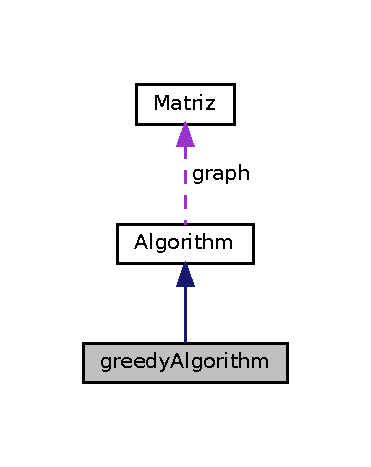
\includegraphics[width=178pt]{classgreedyAlgorithm__coll__graph}
\end{center}
\end{figure}
\subsection*{Public Member Functions}
\begin{DoxyCompactItemize}
\item 
\hyperlink{classgreedyAlgorithm_ad2ec161ba440c1a8f35b26823e37ca6b}{greedy\+Algorithm} (std\+::string filename, int sol)
\begin{DoxyCompactList}\small\item\em Construct a new greedy \hyperlink{classAlgorithm}{Algorithm} object. \end{DoxyCompactList}\item 
std\+::vector$<$ int $>$ \hyperlink{classgreedyAlgorithm_a37c81600b24a32ae25b6f0eeab643a7a}{execute} ()
\begin{DoxyCompactList}\small\item\em Method that executes the algorithm. \end{DoxyCompactList}\item 
std\+::vector$<$ float $>$ \hyperlink{classgreedyAlgorithm_a1ba2f9ae707c3d68f0af86ea320f80cf}{gravity\+Center} (std\+::vector$<$ int $>$)
\begin{DoxyCompactList}\small\item\em Method that calculates the gravity center. \end{DoxyCompactList}\item 
int \hyperlink{classgreedyAlgorithm_afb8dddb24fefb88da82011db8c07e17c}{furthest\+Element} (std\+::vector$<$ int $>$, std\+::vector$<$ float $>$)
\begin{DoxyCompactList}\small\item\em Returns the index of the furthest element to the center. \end{DoxyCompactList}\item 
float \hyperlink{classgreedyAlgorithm_a523e81ad05f34731d5259e712b0b6ee5}{total\+Distance} (std\+::vector$<$ int $>$)
\begin{DoxyCompactList}\small\item\em Method that computes the total distance given a solution. \end{DoxyCompactList}\item 
float \hyperlink{classgreedyAlgorithm_a59dd977d1c232276b8494de999e415d4}{distance\+Two\+Points} (int, int)
\begin{DoxyCompactList}\small\item\em Calculates the distance between two points. \end{DoxyCompactList}\end{DoxyCompactItemize}
\subsection*{Additional Inherited Members}


\subsection{Detailed Description}
Implementation of the greedy algorithm to solve Maximum diversity problem. 

\subsection{Constructor \& Destructor Documentation}
\mbox{\Hypertarget{classgreedyAlgorithm_ad2ec161ba440c1a8f35b26823e37ca6b}\label{classgreedyAlgorithm_ad2ec161ba440c1a8f35b26823e37ca6b}} 
\index{greedy\+Algorithm@{greedy\+Algorithm}!greedy\+Algorithm@{greedy\+Algorithm}}
\index{greedy\+Algorithm@{greedy\+Algorithm}!greedy\+Algorithm@{greedy\+Algorithm}}
\subsubsection{\texorpdfstring{greedy\+Algorithm()}{greedyAlgorithm()}}
{\footnotesize\ttfamily greedy\+Algorithm\+::greedy\+Algorithm (\begin{DoxyParamCaption}\item[{std\+::string}]{filename,  }\item[{int}]{sol }\end{DoxyParamCaption})\hspace{0.3cm}{\ttfamily [inline]}}



Construct a new greedy \hyperlink{classAlgorithm}{Algorithm} object. 


\begin{DoxyParams}{Parameters}
{\em filename} & \\
\hline
\end{DoxyParams}

\begin{DoxyCode}
31 : \hyperlink{classAlgorithm_a3c199c8528aae86f06ac515d5102fa09}{Algorithm}(filename, sol) \{\}
\end{DoxyCode}
Here is the call graph for this function\+:
\nopagebreak
\begin{figure}[H]
\begin{center}
\leavevmode
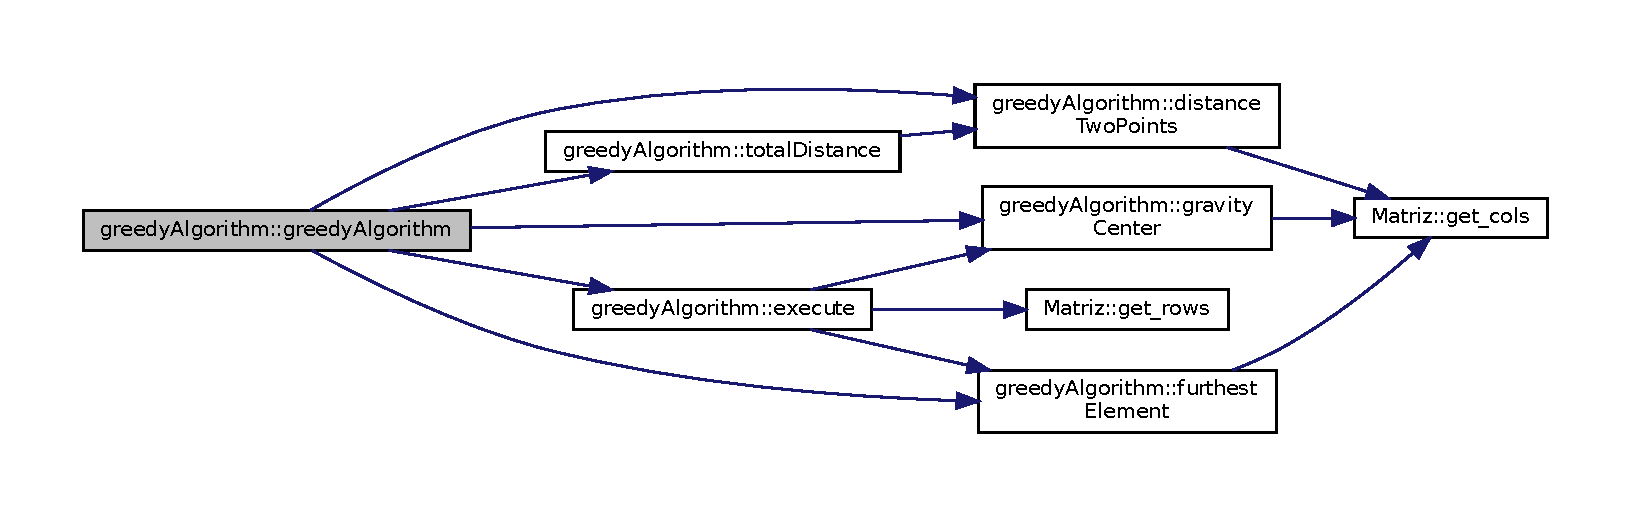
\includegraphics[width=350pt]{classgreedyAlgorithm_ad2ec161ba440c1a8f35b26823e37ca6b_cgraph}
\end{center}
\end{figure}


\subsection{Member Function Documentation}
\mbox{\Hypertarget{classgreedyAlgorithm_a59dd977d1c232276b8494de999e415d4}\label{classgreedyAlgorithm_a59dd977d1c232276b8494de999e415d4}} 
\index{greedy\+Algorithm@{greedy\+Algorithm}!distance\+Two\+Points@{distance\+Two\+Points}}
\index{distance\+Two\+Points@{distance\+Two\+Points}!greedy\+Algorithm@{greedy\+Algorithm}}
\subsubsection{\texorpdfstring{distance\+Two\+Points()}{distanceTwoPoints()}}
{\footnotesize\ttfamily float greedy\+Algorithm\+::distance\+Two\+Points (\begin{DoxyParamCaption}\item[{int}]{point1,  }\item[{int}]{point2 }\end{DoxyParamCaption})}



Calculates the distance between two points. 

\begin{DoxyReturn}{Returns}
float 
\end{DoxyReturn}

\begin{DoxyCode}
70                                                                \{
71   \textcolor{keywordtype}{float} sum = 0; 
72   \textcolor{keywordflow}{for}(\textcolor{keywordtype}{int} j = 0; j < graph.\hyperlink{classMatriz_ad6915f9b31f93230a3ce05d01d23a47b}{get\_cols}(); j++) \{
73     sum += pow(graph[point1][j] - graph[point2][j], 2);
74   \}
75   sum = sqrt(sum);
76   \textcolor{keywordflow}{return} sum;
77 \}
\end{DoxyCode}
Here is the call graph for this function\+:
\nopagebreak
\begin{figure}[H]
\begin{center}
\leavevmode
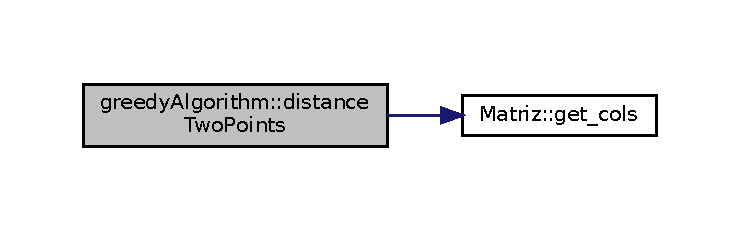
\includegraphics[width=350pt]{classgreedyAlgorithm_a59dd977d1c232276b8494de999e415d4_cgraph}
\end{center}
\end{figure}
Here is the caller graph for this function\+:
\nopagebreak
\begin{figure}[H]
\begin{center}
\leavevmode
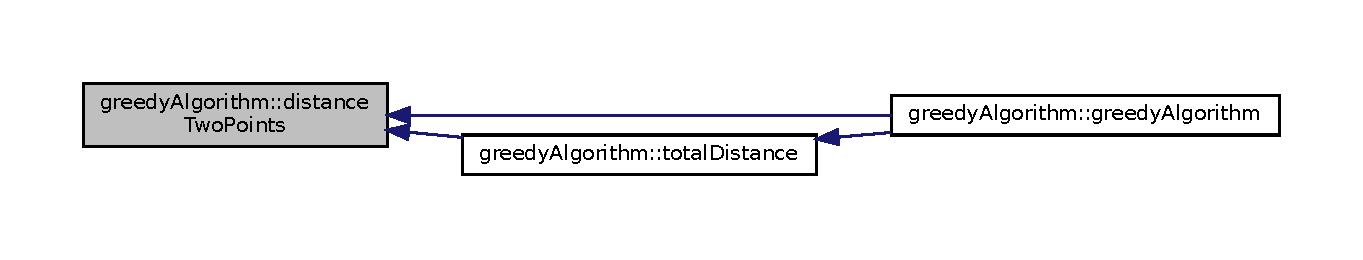
\includegraphics[width=350pt]{classgreedyAlgorithm_a59dd977d1c232276b8494de999e415d4_icgraph}
\end{center}
\end{figure}
\mbox{\Hypertarget{classgreedyAlgorithm_a37c81600b24a32ae25b6f0eeab643a7a}\label{classgreedyAlgorithm_a37c81600b24a32ae25b6f0eeab643a7a}} 
\index{greedy\+Algorithm@{greedy\+Algorithm}!execute@{execute}}
\index{execute@{execute}!greedy\+Algorithm@{greedy\+Algorithm}}
\subsubsection{\texorpdfstring{execute()}{execute()}}
{\footnotesize\ttfamily std\+::vector$<$ int $>$ greedy\+Algorithm\+::execute (\begin{DoxyParamCaption}{ }\end{DoxyParamCaption})\hspace{0.3cm}{\ttfamily [virtual]}}



Method that executes the algorithm. 

\begin{DoxyReturn}{Returns}
std\+::vector$<$float$>$ 
\end{DoxyReturn}


Implements \hyperlink{classAlgorithm_af6ea9eb9a6dbd41896e3fd7dabac096b}{Algorithm}.


\begin{DoxyCode}
4 \{
5   std::vector<int> Elem;
6   std::vector<int> solution;
7   \textcolor{keywordflow}{for} (\textcolor{keywordtype}{int} i = 0; i < graph.\hyperlink{classMatriz_a6b18342f8c083baece693ff41185a206}{get\_rows}(); i++)
8   \{
9     Elem.push\_back(i);
10   \}
11   std::vector<float> SC = \hyperlink{classgreedyAlgorithm_a1ba2f9ae707c3d68f0af86ea320f80cf}{gravityCenter}(Elem);
12   \textcolor{keywordflow}{while}(solution.size() != solutionSize) \{
13     \textcolor{keywordtype}{int} far = \hyperlink{classgreedyAlgorithm_afb8dddb24fefb88da82011db8c07e17c}{furthestElement}(Elem, SC);
14     solution.push\_back(far);
15     Elem.erase(std::find(Elem.begin(), Elem.end(), far));
16     SC = \hyperlink{classgreedyAlgorithm_a1ba2f9ae707c3d68f0af86ea320f80cf}{gravityCenter}(solution);
17   \}
18   \textcolor{keywordflow}{return} solution;
19 \}
\end{DoxyCode}
Here is the call graph for this function\+:
\nopagebreak
\begin{figure}[H]
\begin{center}
\leavevmode
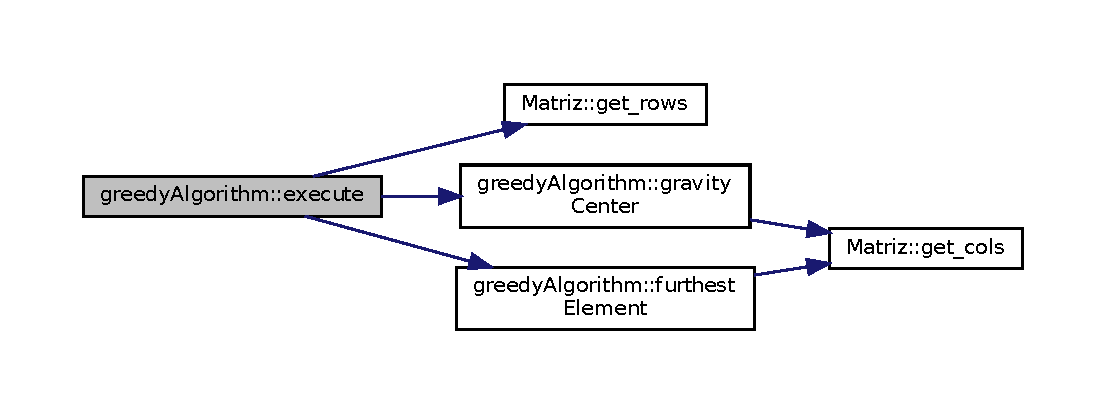
\includegraphics[width=350pt]{classgreedyAlgorithm_a37c81600b24a32ae25b6f0eeab643a7a_cgraph}
\end{center}
\end{figure}
Here is the caller graph for this function\+:
\nopagebreak
\begin{figure}[H]
\begin{center}
\leavevmode
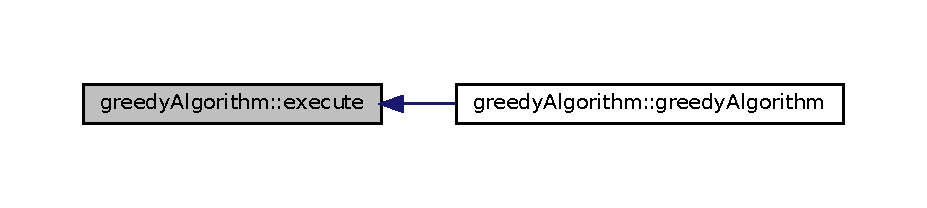
\includegraphics[width=350pt]{classgreedyAlgorithm_a37c81600b24a32ae25b6f0eeab643a7a_icgraph}
\end{center}
\end{figure}
\mbox{\Hypertarget{classgreedyAlgorithm_afb8dddb24fefb88da82011db8c07e17c}\label{classgreedyAlgorithm_afb8dddb24fefb88da82011db8c07e17c}} 
\index{greedy\+Algorithm@{greedy\+Algorithm}!furthest\+Element@{furthest\+Element}}
\index{furthest\+Element@{furthest\+Element}!greedy\+Algorithm@{greedy\+Algorithm}}
\subsubsection{\texorpdfstring{furthest\+Element()}{furthestElement()}}
{\footnotesize\ttfamily int greedy\+Algorithm\+::furthest\+Element (\begin{DoxyParamCaption}\item[{std\+::vector$<$ int $>$}]{Elem,  }\item[{std\+::vector$<$ float $>$}]{SC }\end{DoxyParamCaption})}



Returns the index of the furthest element to the center. 

\begin{DoxyReturn}{Returns}
int 
\end{DoxyReturn}

\begin{DoxyCode}
33                                                                              \{
34   \textcolor{keywordtype}{float} distance = 0;
35   \textcolor{keywordtype}{int} solution = 0;
36   std::vector<int> repetidos;
37   \textcolor{keywordflow}{for}(\textcolor{keywordtype}{int} i = 0; i < Elem.size(); i++) \{
38     \textcolor{keywordtype}{float} sum = 0;
39     \textcolor{keywordflow}{for}(\textcolor{keywordtype}{int} j = 0; j < graph.\hyperlink{classMatriz_ad6915f9b31f93230a3ce05d01d23a47b}{get\_cols}(); j++) \{
40       sum += pow(SC[j] - graph[Elem[i]][j], 2);
41     \}
42     sum = sqrt(sum);
43     \textcolor{keywordflow}{if}(sum > distance) \{
44       distance = sum;
45       solution = Elem[i];
46       repetidos.clear();
47       repetidos.push\_back(Elem[i]);
48     \} \textcolor{keywordflow}{else} \textcolor{keywordflow}{if}(sum == distance) \{
49       repetidos.push\_back(Elem[i]);
50     \}
51   \}
52   \textcolor{keywordflow}{if}(repetidos.size() > 1) \{
53     \textcolor{keywordtype}{int} index = std::rand() % repetidos.size();
54     \textcolor{keywordflow}{return} repetidos[index];
55   \}
56   \textcolor{keywordflow}{return} solution;
57 \}
\end{DoxyCode}
Here is the call graph for this function\+:
\nopagebreak
\begin{figure}[H]
\begin{center}
\leavevmode
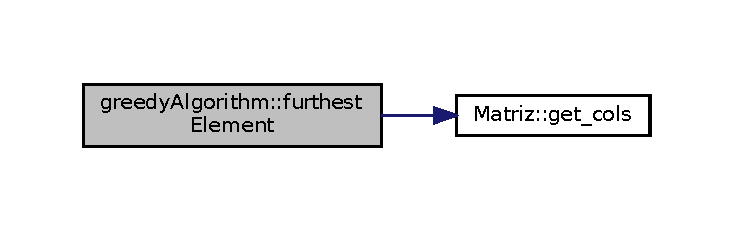
\includegraphics[width=350pt]{classgreedyAlgorithm_afb8dddb24fefb88da82011db8c07e17c_cgraph}
\end{center}
\end{figure}
Here is the caller graph for this function\+:
\nopagebreak
\begin{figure}[H]
\begin{center}
\leavevmode
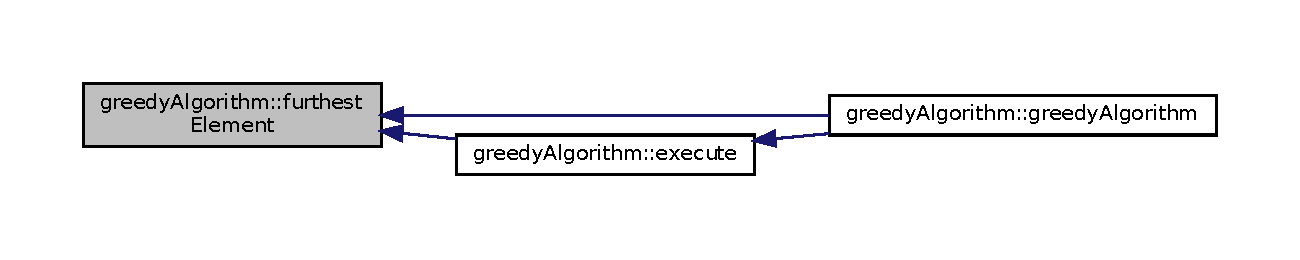
\includegraphics[width=350pt]{classgreedyAlgorithm_afb8dddb24fefb88da82011db8c07e17c_icgraph}
\end{center}
\end{figure}
\mbox{\Hypertarget{classgreedyAlgorithm_a1ba2f9ae707c3d68f0af86ea320f80cf}\label{classgreedyAlgorithm_a1ba2f9ae707c3d68f0af86ea320f80cf}} 
\index{greedy\+Algorithm@{greedy\+Algorithm}!gravity\+Center@{gravity\+Center}}
\index{gravity\+Center@{gravity\+Center}!greedy\+Algorithm@{greedy\+Algorithm}}
\subsubsection{\texorpdfstring{gravity\+Center()}{gravityCenter()}}
{\footnotesize\ttfamily std\+::vector$<$ float $>$ greedy\+Algorithm\+::gravity\+Center (\begin{DoxyParamCaption}\item[{std\+::vector$<$ int $>$}]{Elem }\end{DoxyParamCaption})}



Method that calculates the gravity center. 

\begin{DoxyReturn}{Returns}
std\+::vector$<$float$>$ 
\end{DoxyReturn}

\begin{DoxyCode}
21                                                                    \{
22   std::vector<float> solution;
23   \textcolor{keywordflow}{for}(\textcolor{keywordtype}{int} i = 0; i < graph.\hyperlink{classMatriz_ad6915f9b31f93230a3ce05d01d23a47b}{get\_cols}(); i++) \{
24     \textcolor{keywordtype}{float} sum = 0;
25     \textcolor{keywordflow}{for}(\textcolor{keywordtype}{int} j = 0; j < Elem.size(); j++) \{      
26       sum += graph[Elem[j]][i]; 
27     \}
28     solution.push\_back(sum / Elem.size());
29   \}
30   \textcolor{keywordflow}{return} solution;
31 \}
\end{DoxyCode}
Here is the call graph for this function\+:
\nopagebreak
\begin{figure}[H]
\begin{center}
\leavevmode
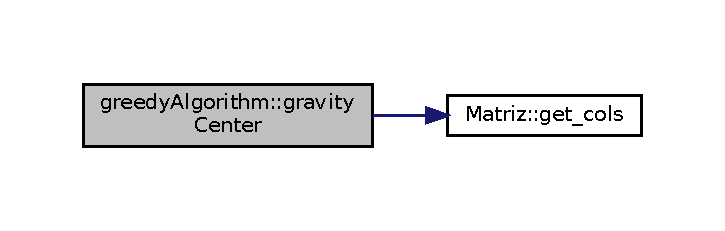
\includegraphics[width=348pt]{classgreedyAlgorithm_a1ba2f9ae707c3d68f0af86ea320f80cf_cgraph}
\end{center}
\end{figure}
Here is the caller graph for this function\+:
\nopagebreak
\begin{figure}[H]
\begin{center}
\leavevmode
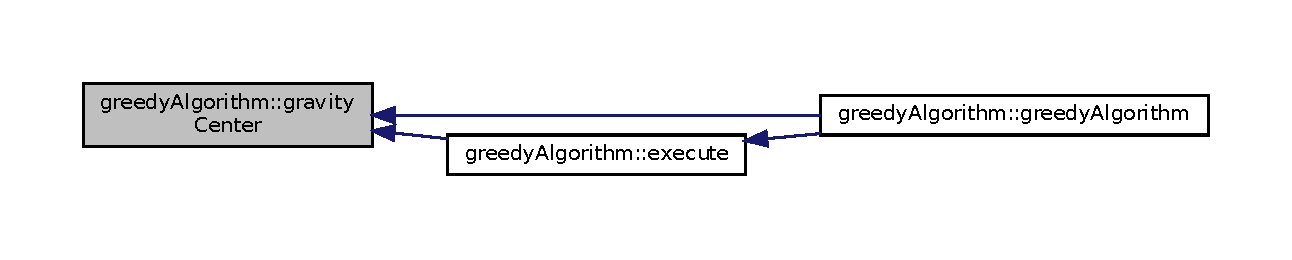
\includegraphics[width=350pt]{classgreedyAlgorithm_a1ba2f9ae707c3d68f0af86ea320f80cf_icgraph}
\end{center}
\end{figure}
\mbox{\Hypertarget{classgreedyAlgorithm_a523e81ad05f34731d5259e712b0b6ee5}\label{classgreedyAlgorithm_a523e81ad05f34731d5259e712b0b6ee5}} 
\index{greedy\+Algorithm@{greedy\+Algorithm}!total\+Distance@{total\+Distance}}
\index{total\+Distance@{total\+Distance}!greedy\+Algorithm@{greedy\+Algorithm}}
\subsubsection{\texorpdfstring{total\+Distance()}{totalDistance()}}
{\footnotesize\ttfamily float greedy\+Algorithm\+::total\+Distance (\begin{DoxyParamCaption}\item[{std\+::vector$<$ int $>$}]{solution }\end{DoxyParamCaption})}



Method that computes the total distance given a solution. 

\begin{DoxyReturn}{Returns}
float 
\end{DoxyReturn}

\begin{DoxyCode}
60                                                             \{
61   \textcolor{keywordtype}{float} sum = 0;
62   \textcolor{keywordflow}{for}(\textcolor{keywordtype}{int} i = 0; i < solution.size(); i++) \{
63     \textcolor{keywordflow}{for}(\textcolor{keywordtype}{int} j = i + 1; j < solution.size(); j++) \{
64       sum += \hyperlink{classgreedyAlgorithm_a59dd977d1c232276b8494de999e415d4}{distanceTwoPoints}(solution[i], solution[j]);
65     \}
66   \}
67   \textcolor{keywordflow}{return} sum;
68 \}
\end{DoxyCode}
Here is the call graph for this function\+:
\nopagebreak
\begin{figure}[H]
\begin{center}
\leavevmode
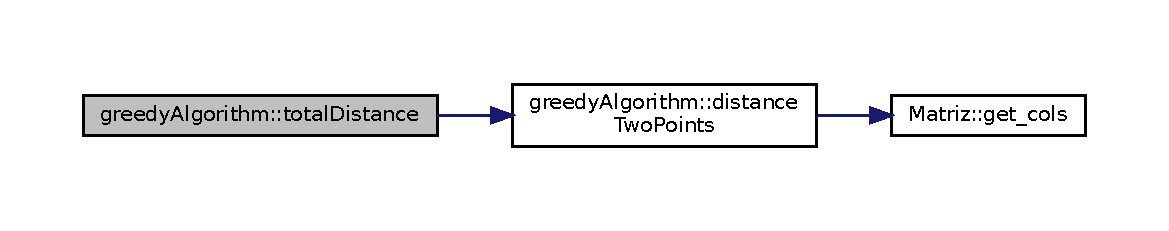
\includegraphics[width=350pt]{classgreedyAlgorithm_a523e81ad05f34731d5259e712b0b6ee5_cgraph}
\end{center}
\end{figure}
Here is the caller graph for this function\+:
\nopagebreak
\begin{figure}[H]
\begin{center}
\leavevmode
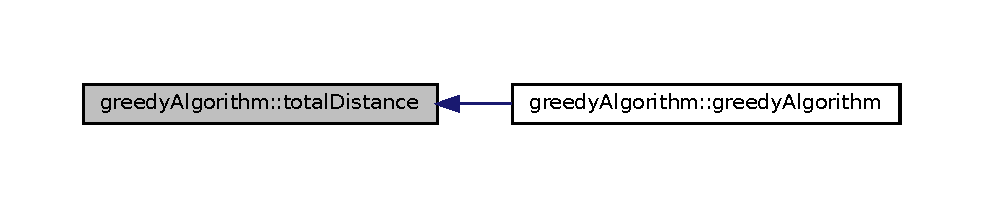
\includegraphics[width=350pt]{classgreedyAlgorithm_a523e81ad05f34731d5259e712b0b6ee5_icgraph}
\end{center}
\end{figure}


The documentation for this class was generated from the following files\+:\begin{DoxyCompactItemize}
\item 
include/\hyperlink{greedyAlgorithm_8hpp}{greedy\+Algorithm.\+hpp}\item 
src/greedy\+Algorithm.\+cpp\end{DoxyCompactItemize}

\hypertarget{classlocalSearch}{}\section{local\+Search Class Reference}
\label{classlocalSearch}\index{local\+Search@{local\+Search}}


Implementation of the Local Search algorithm.  




{\ttfamily \#include $<$local\+Search.\+hpp$>$}



Inheritance diagram for local\+Search\+:
\nopagebreak
\begin{figure}[H]
\begin{center}
\leavevmode
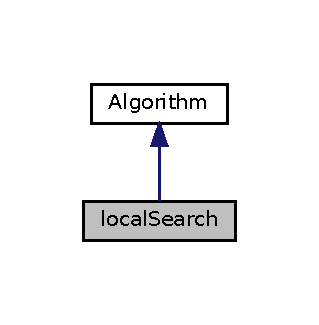
\includegraphics[width=153pt]{classlocalSearch__inherit__graph}
\end{center}
\end{figure}


Collaboration diagram for local\+Search\+:
\nopagebreak
\begin{figure}[H]
\begin{center}
\leavevmode
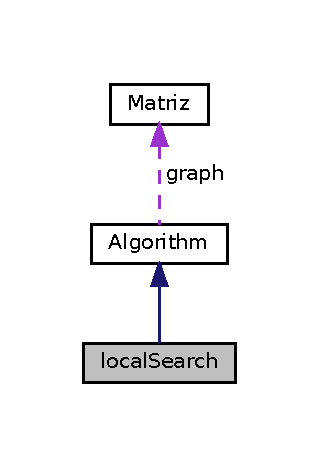
\includegraphics[width=153pt]{classlocalSearch__coll__graph}
\end{center}
\end{figure}
\subsection*{Public Member Functions}
\begin{DoxyCompactItemize}
\item 
\hyperlink{classlocalSearch_a30b47bf0168e1ad75f42868780de1f96}{local\+Search} (std\+::string filename, int sol, std\+::vector$<$ int $>$ solution\+Greedy)
\begin{DoxyCompactList}\small\item\em Construct a new \hyperlink{classlocalSearch}{local\+Search} object. \end{DoxyCompactList}\item 
std\+::vector$<$ int $>$ \hyperlink{classlocalSearch_a0ac1d7bf221f1ab7af92f1a91017cf02}{execute} ()
\begin{DoxyCompactList}\small\item\em Method that executes the algorithm. \end{DoxyCompactList}\item 
std\+::vector$<$ int $>$ \hyperlink{classlocalSearch_afe2b71349ac06285bdccaf85847650c0}{local\+\_\+\+Search} (std\+::vector$<$ int $>$ solution)
\begin{DoxyCompactList}\small\item\em Returns the a vector with the improved solution after applying the local search algorithm. \end{DoxyCompactList}\item 
float \hyperlink{classlocalSearch_a0b14e5f24760de3ea567ff507d3a2ece}{total\+Distance} (std\+::vector$<$ int $>$)
\begin{DoxyCompactList}\small\item\em Method that computes the total distance given a solution. \end{DoxyCompactList}\item 
float \hyperlink{classlocalSearch_a5e85839cfb397c2ee38fa38bfbbc4151}{distance\+Two\+Points} (int, int)
\begin{DoxyCompactList}\small\item\em Calculates the distance between two points. \end{DoxyCompactList}\end{DoxyCompactItemize}
\subsection*{Additional Inherited Members}


\subsection{Detailed Description}
Implementation of the Local Search algorithm. 

\subsection{Constructor \& Destructor Documentation}
\mbox{\Hypertarget{classlocalSearch_a30b47bf0168e1ad75f42868780de1f96}\label{classlocalSearch_a30b47bf0168e1ad75f42868780de1f96}} 
\index{local\+Search@{local\+Search}!local\+Search@{local\+Search}}
\index{local\+Search@{local\+Search}!local\+Search@{local\+Search}}
\subsubsection{\texorpdfstring{local\+Search()}{localSearch()}}
{\footnotesize\ttfamily local\+Search\+::local\+Search (\begin{DoxyParamCaption}\item[{std\+::string}]{filename,  }\item[{int}]{sol,  }\item[{std\+::vector$<$ int $>$}]{solution\+Greedy }\end{DoxyParamCaption})\hspace{0.3cm}{\ttfamily [inline]}}



Construct a new \hyperlink{classlocalSearch}{local\+Search} object. 


\begin{DoxyParams}{Parameters}
{\em filename} & \\
\hline
\end{DoxyParams}

\begin{DoxyCode}
30 : \hyperlink{classAlgorithm_a3c199c8528aae86f06ac515d5102fa09}{Algorithm}(filename, sol), solutionGreedy(solutionGreedy) \{\}
\end{DoxyCode}
Here is the call graph for this function\+:
\nopagebreak
\begin{figure}[H]
\begin{center}
\leavevmode
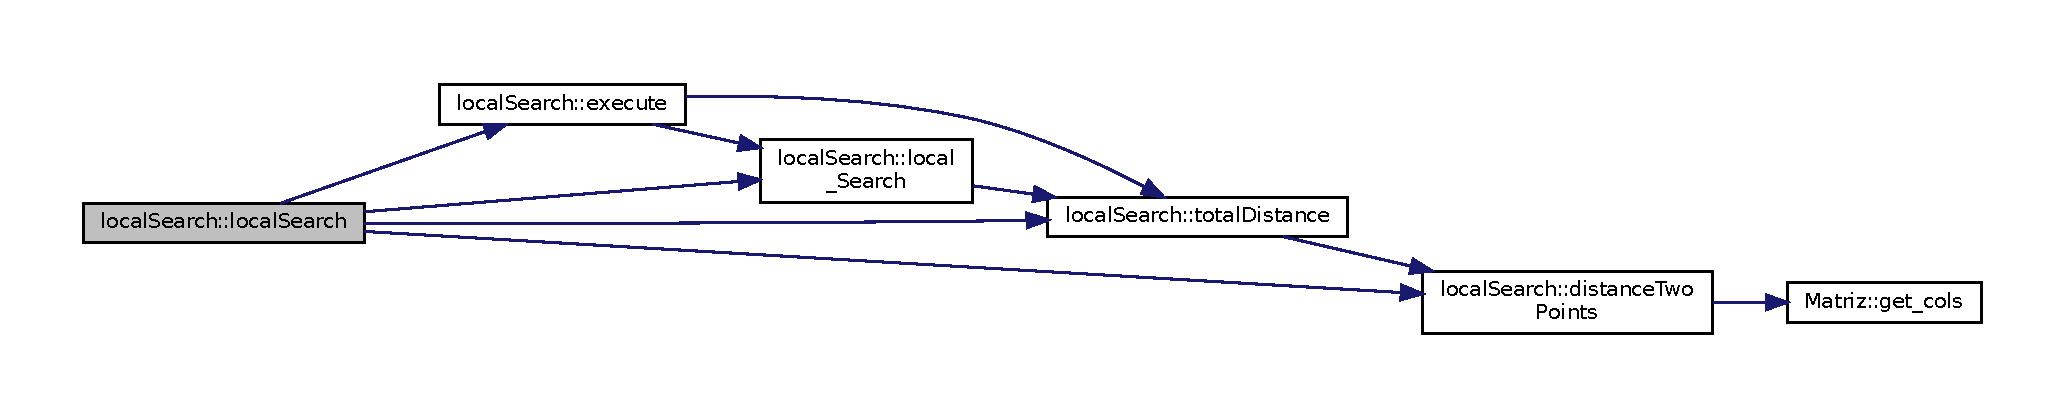
\includegraphics[width=350pt]{classlocalSearch_a30b47bf0168e1ad75f42868780de1f96_cgraph}
\end{center}
\end{figure}


\subsection{Member Function Documentation}
\mbox{\Hypertarget{classlocalSearch_a5e85839cfb397c2ee38fa38bfbbc4151}\label{classlocalSearch_a5e85839cfb397c2ee38fa38bfbbc4151}} 
\index{local\+Search@{local\+Search}!distance\+Two\+Points@{distance\+Two\+Points}}
\index{distance\+Two\+Points@{distance\+Two\+Points}!local\+Search@{local\+Search}}
\subsubsection{\texorpdfstring{distance\+Two\+Points()}{distanceTwoPoints()}}
{\footnotesize\ttfamily float local\+Search\+::distance\+Two\+Points (\begin{DoxyParamCaption}\item[{int}]{point1,  }\item[{int}]{point2 }\end{DoxyParamCaption})}



Calculates the distance between two points. 

\begin{DoxyReturn}{Returns}
float 
\end{DoxyReturn}

\begin{DoxyCode}
61                                                            \{
62   \textcolor{keywordtype}{float} sum = 0; 
63   \textcolor{keywordflow}{for}(\textcolor{keywordtype}{int} j = 0; j < graph.\hyperlink{classMatriz_ad6915f9b31f93230a3ce05d01d23a47b}{get\_cols}(); j++) \{
64     sum += pow(graph[point1][j] - graph[point2][j], 2);
65   \}
66   sum = sqrt(sum);
67   \textcolor{keywordflow}{return} sum;
68 \}
\end{DoxyCode}
Here is the call graph for this function\+:
\nopagebreak
\begin{figure}[H]
\begin{center}
\leavevmode
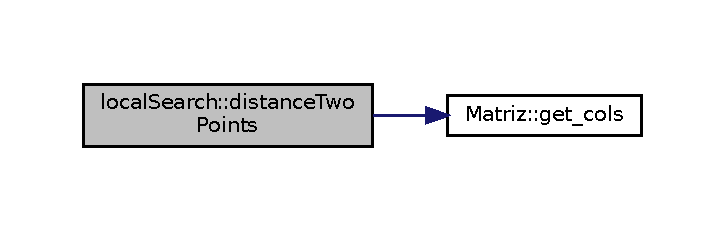
\includegraphics[width=348pt]{classlocalSearch_a5e85839cfb397c2ee38fa38bfbbc4151_cgraph}
\end{center}
\end{figure}
Here is the caller graph for this function\+:
\nopagebreak
\begin{figure}[H]
\begin{center}
\leavevmode
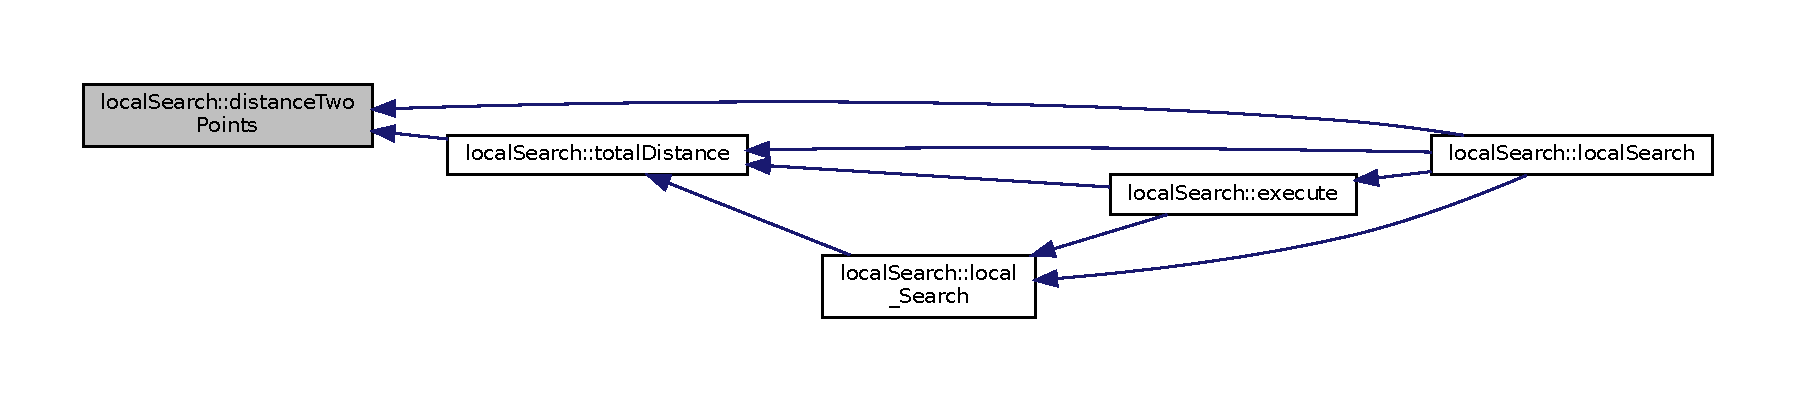
\includegraphics[width=350pt]{classlocalSearch_a5e85839cfb397c2ee38fa38bfbbc4151_icgraph}
\end{center}
\end{figure}
\mbox{\Hypertarget{classlocalSearch_a0ac1d7bf221f1ab7af92f1a91017cf02}\label{classlocalSearch_a0ac1d7bf221f1ab7af92f1a91017cf02}} 
\index{local\+Search@{local\+Search}!execute@{execute}}
\index{execute@{execute}!local\+Search@{local\+Search}}
\subsubsection{\texorpdfstring{execute()}{execute()}}
{\footnotesize\ttfamily std\+::vector$<$ int $>$ local\+Search\+::execute (\begin{DoxyParamCaption}{ }\end{DoxyParamCaption})\hspace{0.3cm}{\ttfamily [virtual]}}



Method that executes the algorithm. 

\begin{DoxyReturn}{Returns}
std\+::vector$<$float$>$ 
\end{DoxyReturn}


Implements \hyperlink{classAlgorithm_af6ea9eb9a6dbd41896e3fd7dabac096b}{Algorithm}.


\begin{DoxyCode}
3 \{
4   std::vector<int> solution = solutionGreedy;
5   \textcolor{keywordtype}{float} distance = \hyperlink{classlocalSearch_a0b14e5f24760de3ea567ff507d3a2ece}{totalDistance}(solution);
6   \textcolor{keywordtype}{bool} improvement = \textcolor{keyword}{true};
7   \textcolor{keywordflow}{if}(improvement) \{
8     std::vector<int> improvedSolution = \hyperlink{classlocalSearch_afe2b71349ac06285bdccaf85847650c0}{local\_Search}(solution);
9     \textcolor{keywordflow}{if}(\hyperlink{classlocalSearch_a0b14e5f24760de3ea567ff507d3a2ece}{totalDistance}(improvedSolution) > distance) \{
10       solution = improvedSolution;
11       distance = \hyperlink{classlocalSearch_a0b14e5f24760de3ea567ff507d3a2ece}{totalDistance}(improvedSolution);
12     \} \textcolor{keywordflow}{else} \{
13       improvement = \textcolor{keyword}{false};
14     \}
15   \}
16   \textcolor{keywordflow}{return} solution;
17 \}
\end{DoxyCode}
Here is the call graph for this function\+:
\nopagebreak
\begin{figure}[H]
\begin{center}
\leavevmode
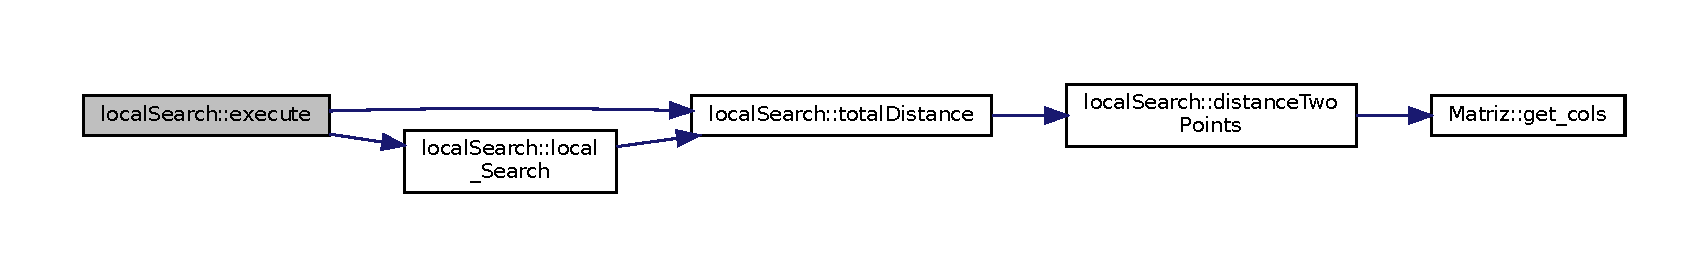
\includegraphics[width=350pt]{classlocalSearch_a0ac1d7bf221f1ab7af92f1a91017cf02_cgraph}
\end{center}
\end{figure}
Here is the caller graph for this function\+:
\nopagebreak
\begin{figure}[H]
\begin{center}
\leavevmode

\includegraphics[width=350pt]{classlocalSearch_a0ac1d7bf221f1ab7af92f1a91017cf02_icgraph}
\end{center}
\end{figure}
\mbox{\Hypertarget{classlocalSearch_afe2b71349ac06285bdccaf85847650c0}\label{classlocalSearch_afe2b71349ac06285bdccaf85847650c0}} 
\index{local\+Search@{local\+Search}!local\+\_\+\+Search@{local\+\_\+\+Search}}
\index{local\+\_\+\+Search@{local\+\_\+\+Search}!local\+Search@{local\+Search}}
\subsubsection{\texorpdfstring{local\+\_\+\+Search()}{local\_Search()}}
{\footnotesize\ttfamily std\+::vector$<$ int $>$ local\+Search\+::local\+\_\+\+Search (\begin{DoxyParamCaption}\item[{std\+::vector$<$ int $>$}]{solution }\end{DoxyParamCaption})}



Returns the a vector with the improved solution after applying the local search algorithm. 


\begin{DoxyParams}{Parameters}
{\em solution} & \\
\hline
\end{DoxyParams}
\begin{DoxyReturn}{Returns}
std\+::vector$<$int$>$ 
\end{DoxyReturn}

\begin{DoxyCode}
21 \{
22   \textcolor{keywordtype}{float} distance = \hyperlink{classlocalSearch_a0b14e5f24760de3ea567ff507d3a2ece}{totalDistance}(solutionGreedy);
23   std::vector<int> improved;
24   std::vector<int> actualSolution = solutionGreedy;
25   std::vector<int> candidates;
26   \textcolor{keywordtype}{bool} improv = \textcolor{keyword}{false};
27   \textcolor{keywordflow}{do} \{
28     \textcolor{keywordflow}{for}(\textcolor{keywordtype}{int} i = 0; i < solution.size(); i++) \{
29       \textcolor{keywordflow}{if}(std::find(solution.begin(), solution.end(), i) == solution.end()) \{
30         candidates.push\_back(i);
31       \}
32     \}
33     improv = \textcolor{keyword}{false};
34     \textcolor{keywordflow}{for}(\textcolor{keywordtype}{int} i = 0; i < actualSolution.size(); i++) \{
35       \textcolor{keywordtype}{int} aux = actualSolution[i];
36       \textcolor{keywordflow}{for}(\textcolor{keywordtype}{int} j = 0; j < candidates.size(); j++) \{
37         actualSolution[i] = candidates[j];
38         \textcolor{keywordtype}{float} actualDistance = \hyperlink{classlocalSearch_a0b14e5f24760de3ea567ff507d3a2ece}{totalDistance}(actualSolution);
39         \textcolor{keywordflow}{if}(actualDistance > distance) \{
40           distance = actualDistance;
41           improved = actualSolution;
42           improv = \textcolor{keyword}{true};
43         \}
44       \}
45       actualSolution[i] = aux;
46     \}
47   \} \textcolor{keywordflow}{while}(improv);
48   \textcolor{keywordflow}{return} improved;
49 \}
\end{DoxyCode}
Here is the call graph for this function\+:
\nopagebreak
\begin{figure}[H]
\begin{center}
\leavevmode
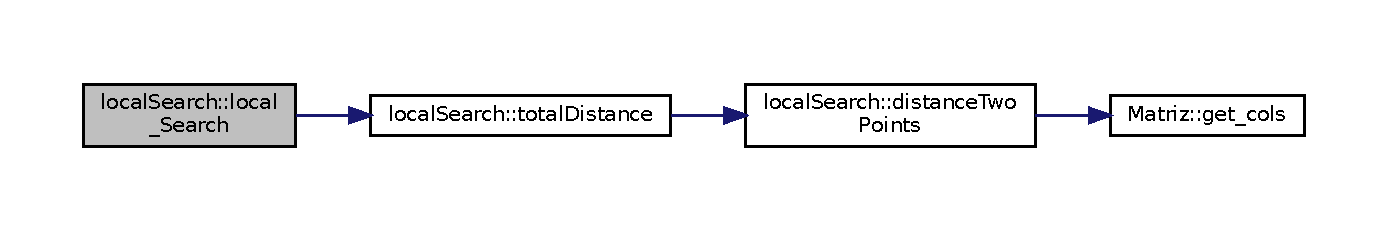
\includegraphics[width=350pt]{classlocalSearch_afe2b71349ac06285bdccaf85847650c0_cgraph}
\end{center}
\end{figure}
Here is the caller graph for this function\+:
\nopagebreak
\begin{figure}[H]
\begin{center}
\leavevmode
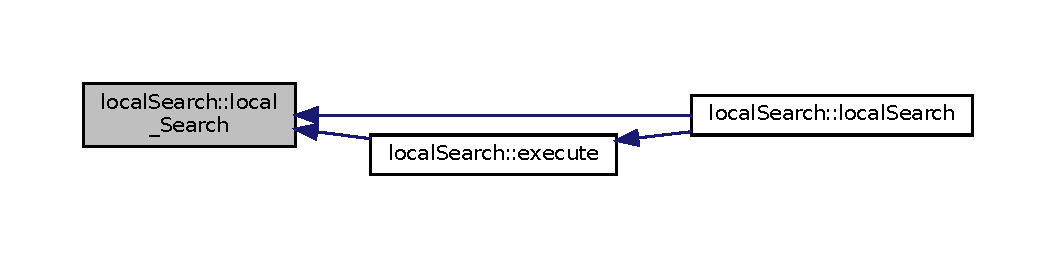
\includegraphics[width=350pt]{classlocalSearch_afe2b71349ac06285bdccaf85847650c0_icgraph}
\end{center}
\end{figure}
\mbox{\Hypertarget{classlocalSearch_a0b14e5f24760de3ea567ff507d3a2ece}\label{classlocalSearch_a0b14e5f24760de3ea567ff507d3a2ece}} 
\index{local\+Search@{local\+Search}!total\+Distance@{total\+Distance}}
\index{total\+Distance@{total\+Distance}!local\+Search@{local\+Search}}
\subsubsection{\texorpdfstring{total\+Distance()}{totalDistance()}}
{\footnotesize\ttfamily float local\+Search\+::total\+Distance (\begin{DoxyParamCaption}\item[{std\+::vector$<$ int $>$}]{solution }\end{DoxyParamCaption})}



Method that computes the total distance given a solution. 

\begin{DoxyReturn}{Returns}
float 
\end{DoxyReturn}

\begin{DoxyCode}
51                                                         \{
52   \textcolor{keywordtype}{float} sum = 0;
53   \textcolor{keywordflow}{for}(\textcolor{keywordtype}{int} i = 0; i < solution.size(); i++) \{
54     \textcolor{keywordflow}{for}(\textcolor{keywordtype}{int} j = i + 1; j < solution.size(); j++) \{
55       sum += \hyperlink{classlocalSearch_a5e85839cfb397c2ee38fa38bfbbc4151}{distanceTwoPoints}(solution[i], solution[j]);
56     \}
57   \}
58   \textcolor{keywordflow}{return} sum;
59 \}
\end{DoxyCode}
Here is the call graph for this function\+:
\nopagebreak
\begin{figure}[H]
\begin{center}
\leavevmode
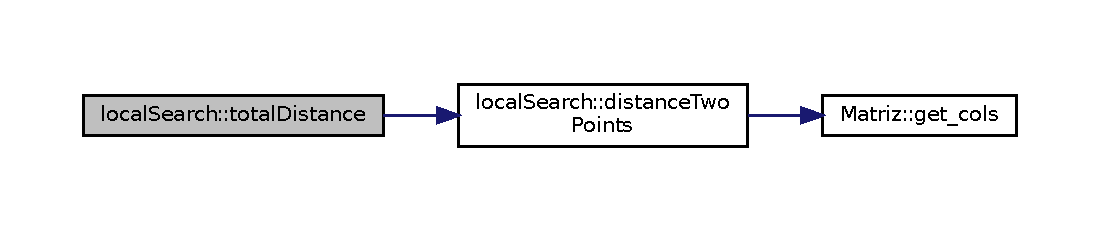
\includegraphics[width=350pt]{classlocalSearch_a0b14e5f24760de3ea567ff507d3a2ece_cgraph}
\end{center}
\end{figure}
Here is the caller graph for this function\+:
\nopagebreak
\begin{figure}[H]
\begin{center}
\leavevmode
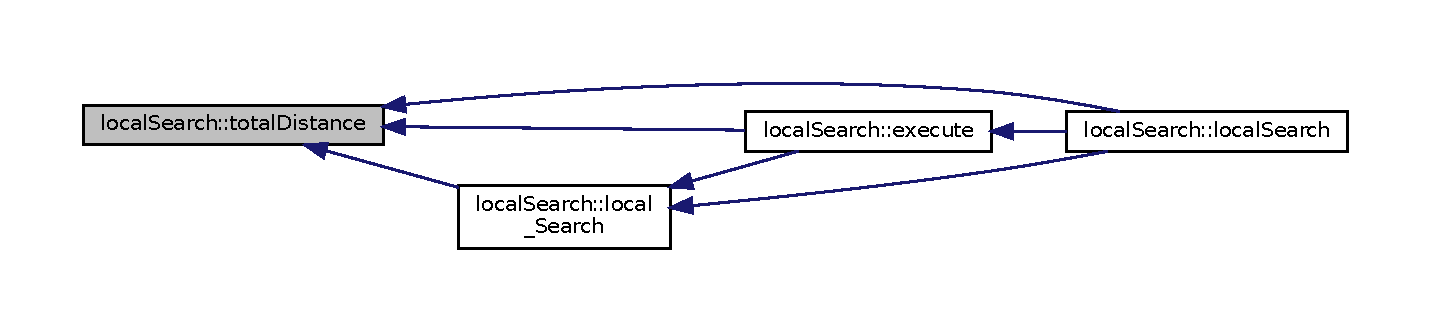
\includegraphics[width=350pt]{classlocalSearch_a0b14e5f24760de3ea567ff507d3a2ece_icgraph}
\end{center}
\end{figure}


The documentation for this class was generated from the following files\+:\begin{DoxyCompactItemize}
\item 
include/\hyperlink{localSearch_8hpp}{local\+Search.\+hpp}\item 
src/local\+Search.\+cpp\end{DoxyCompactItemize}

\hypertarget{classMatriz}{}\section{Matriz Class Reference}
\label{classMatriz}\index{Matriz@{Matriz}}


Matrix containing all the distances between nodes.  




{\ttfamily \#include $<$Matrix.\+hpp$>$}

\subsection*{Public Member Functions}
\begin{DoxyCompactItemize}
\item 
\hyperlink{classMatriz_a388709cfee356a0c78b66e3f538e9318}{Matriz} (std\+::string filename)
\begin{DoxyCompactList}\small\item\em Construct a new \hyperlink{classMatriz}{Matriz} object. \end{DoxyCompactList}\item 
void \hyperlink{classMatriz_aa929f933e9088dc0efecaa9a46d555d9}{resize\+Matrix} (int rows, int cols)
\begin{DoxyCompactList}\small\item\em Change the matrix\textquotesingle{}s dimensions. \end{DoxyCompactList}\item 
int \hyperlink{classMatriz_a6b18342f8c083baece693ff41185a206}{get\+\_\+rows} ()
\begin{DoxyCompactList}\small\item\em Get the rows object. \end{DoxyCompactList}\item 
int \hyperlink{classMatriz_ad6915f9b31f93230a3ce05d01d23a47b}{get\+\_\+cols} ()
\begin{DoxyCompactList}\small\item\em Get the cols object. \end{DoxyCompactList}\item 
void \hyperlink{classMatriz_a3641ea6e8f91cffd9073c22a71082cf8}{set\+\_\+position} (int row, int col, float value)
\begin{DoxyCompactList}\small\item\em Set the position object. \end{DoxyCompactList}\item 
float \hyperlink{classMatriz_aaf1b9c3af2d3b269cc0a2dda08aebd61}{get\+\_\+position} (int row, int col)
\begin{DoxyCompactList}\small\item\em Get the position object. \end{DoxyCompactList}\item 
\mbox{\Hypertarget{classMatriz_ae0fd5f42c3797c8d4b85c1d6701e0e7e}\label{classMatriz_ae0fd5f42c3797c8d4b85c1d6701e0e7e}} 
void \hyperlink{classMatriz_ae0fd5f42c3797c8d4b85c1d6701e0e7e}{write} ()
\begin{DoxyCompactList}\small\item\em Print the matrix. \end{DoxyCompactList}\item 
std\+::vector$<$ float $>$ \& \hyperlink{classMatriz_a5516a9b9524e4604d4b3040628be50e9}{operator\mbox{[}$\,$\mbox{]}} (int index)
\begin{DoxyCompactList}\small\item\em Operator \mbox{[}\mbox{]} overload. \end{DoxyCompactList}\item 
\mbox{\Hypertarget{classMatriz_afa298e352ed08188e16edf49fc49fcc2}\label{classMatriz_afa298e352ed08188e16edf49fc49fcc2}} 
void {\bfseries print\+Row} (int index)
\end{DoxyCompactItemize}


\subsection{Detailed Description}
Matrix containing all the distances between nodes. 

\subsection{Constructor \& Destructor Documentation}
\mbox{\Hypertarget{classMatriz_a388709cfee356a0c78b66e3f538e9318}\label{classMatriz_a388709cfee356a0c78b66e3f538e9318}} 
\index{Matriz@{Matriz}!Matriz@{Matriz}}
\index{Matriz@{Matriz}!Matriz@{Matriz}}
\subsubsection{\texorpdfstring{Matriz()}{Matriz()}}
{\footnotesize\ttfamily Matriz\+::\+Matriz (\begin{DoxyParamCaption}\item[{std\+::string}]{filename }\end{DoxyParamCaption})\hspace{0.3cm}{\ttfamily [inline]}}



Construct a new \hyperlink{classMatriz}{Matriz} object. 


\begin{DoxyParams}{Parameters}
{\em \{std\+::string\}} & filename \\
\hline
\end{DoxyParams}

\begin{DoxyCode}
36                              : matrix(0, std::vector<float>(0))
37   \{
38     std::ifstream myFile;
39     myFile.open(filename);
40     \textcolor{keywordtype}{int} numeroElementos = 0;
41     \textcolor{keywordtype}{int} dimensionElementos = 0;
42     \textcolor{keywordtype}{float} valores = 0;
43     \textcolor{keywordflow}{if} (myFile.is\_open())
44     \{
45       myFile >> numeroElementos;
46       myFile >> dimensionElementos;
47     \}
48     this->\hyperlink{classMatriz_aa929f933e9088dc0efecaa9a46d555d9}{resizeMatrix}(numeroElementos, dimensionElementos);
49     \textcolor{keywordflow}{for} (\textcolor{keywordtype}{int} i = 0; i < numeroElementos; i++)
50     \{
51       \textcolor{keywordflow}{for} (\textcolor{keywordtype}{int} j = 0; j < dimensionElementos; j++)
52       \{
53         matrix[i][j] = 0;
54       \}
55     \}
56     \textcolor{keywordflow}{for} (\textcolor{keywordtype}{int} i = 0; i < numeroElementos; i++)
57     \{
58       \textcolor{keywordflow}{for} (\textcolor{keywordtype}{int} j = 0; j < dimensionElementos; j++)
59       \{
60           myFile >> valores;
61           matrix[i][j] = valores;
62       \}
63     \}
64     myFile.close();
65   \}
\end{DoxyCode}
Here is the call graph for this function\+:
\nopagebreak
\begin{figure}[H]
\begin{center}
\leavevmode
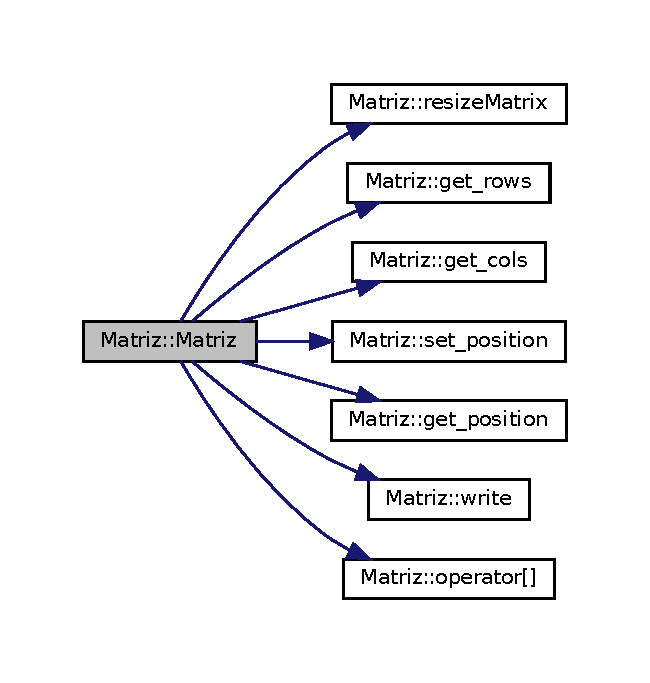
\includegraphics[width=312pt]{classMatriz_a388709cfee356a0c78b66e3f538e9318_cgraph}
\end{center}
\end{figure}


\subsection{Member Function Documentation}
\mbox{\Hypertarget{classMatriz_ad6915f9b31f93230a3ce05d01d23a47b}\label{classMatriz_ad6915f9b31f93230a3ce05d01d23a47b}} 
\index{Matriz@{Matriz}!get\+\_\+cols@{get\+\_\+cols}}
\index{get\+\_\+cols@{get\+\_\+cols}!Matriz@{Matriz}}
\subsubsection{\texorpdfstring{get\+\_\+cols()}{get\_cols()}}
{\footnotesize\ttfamily int Matriz\+::get\+\_\+cols (\begin{DoxyParamCaption}{ }\end{DoxyParamCaption})}



Get the cols object. 

\begin{DoxyReturn}{Returns}
float 
\end{DoxyReturn}

\begin{DoxyCode}
18 \{
19   \textcolor{keywordflow}{return} matrix[0].size();
20 \}
\end{DoxyCode}
Here is the caller graph for this function\+:
\nopagebreak
\begin{figure}[H]
\begin{center}
\leavevmode
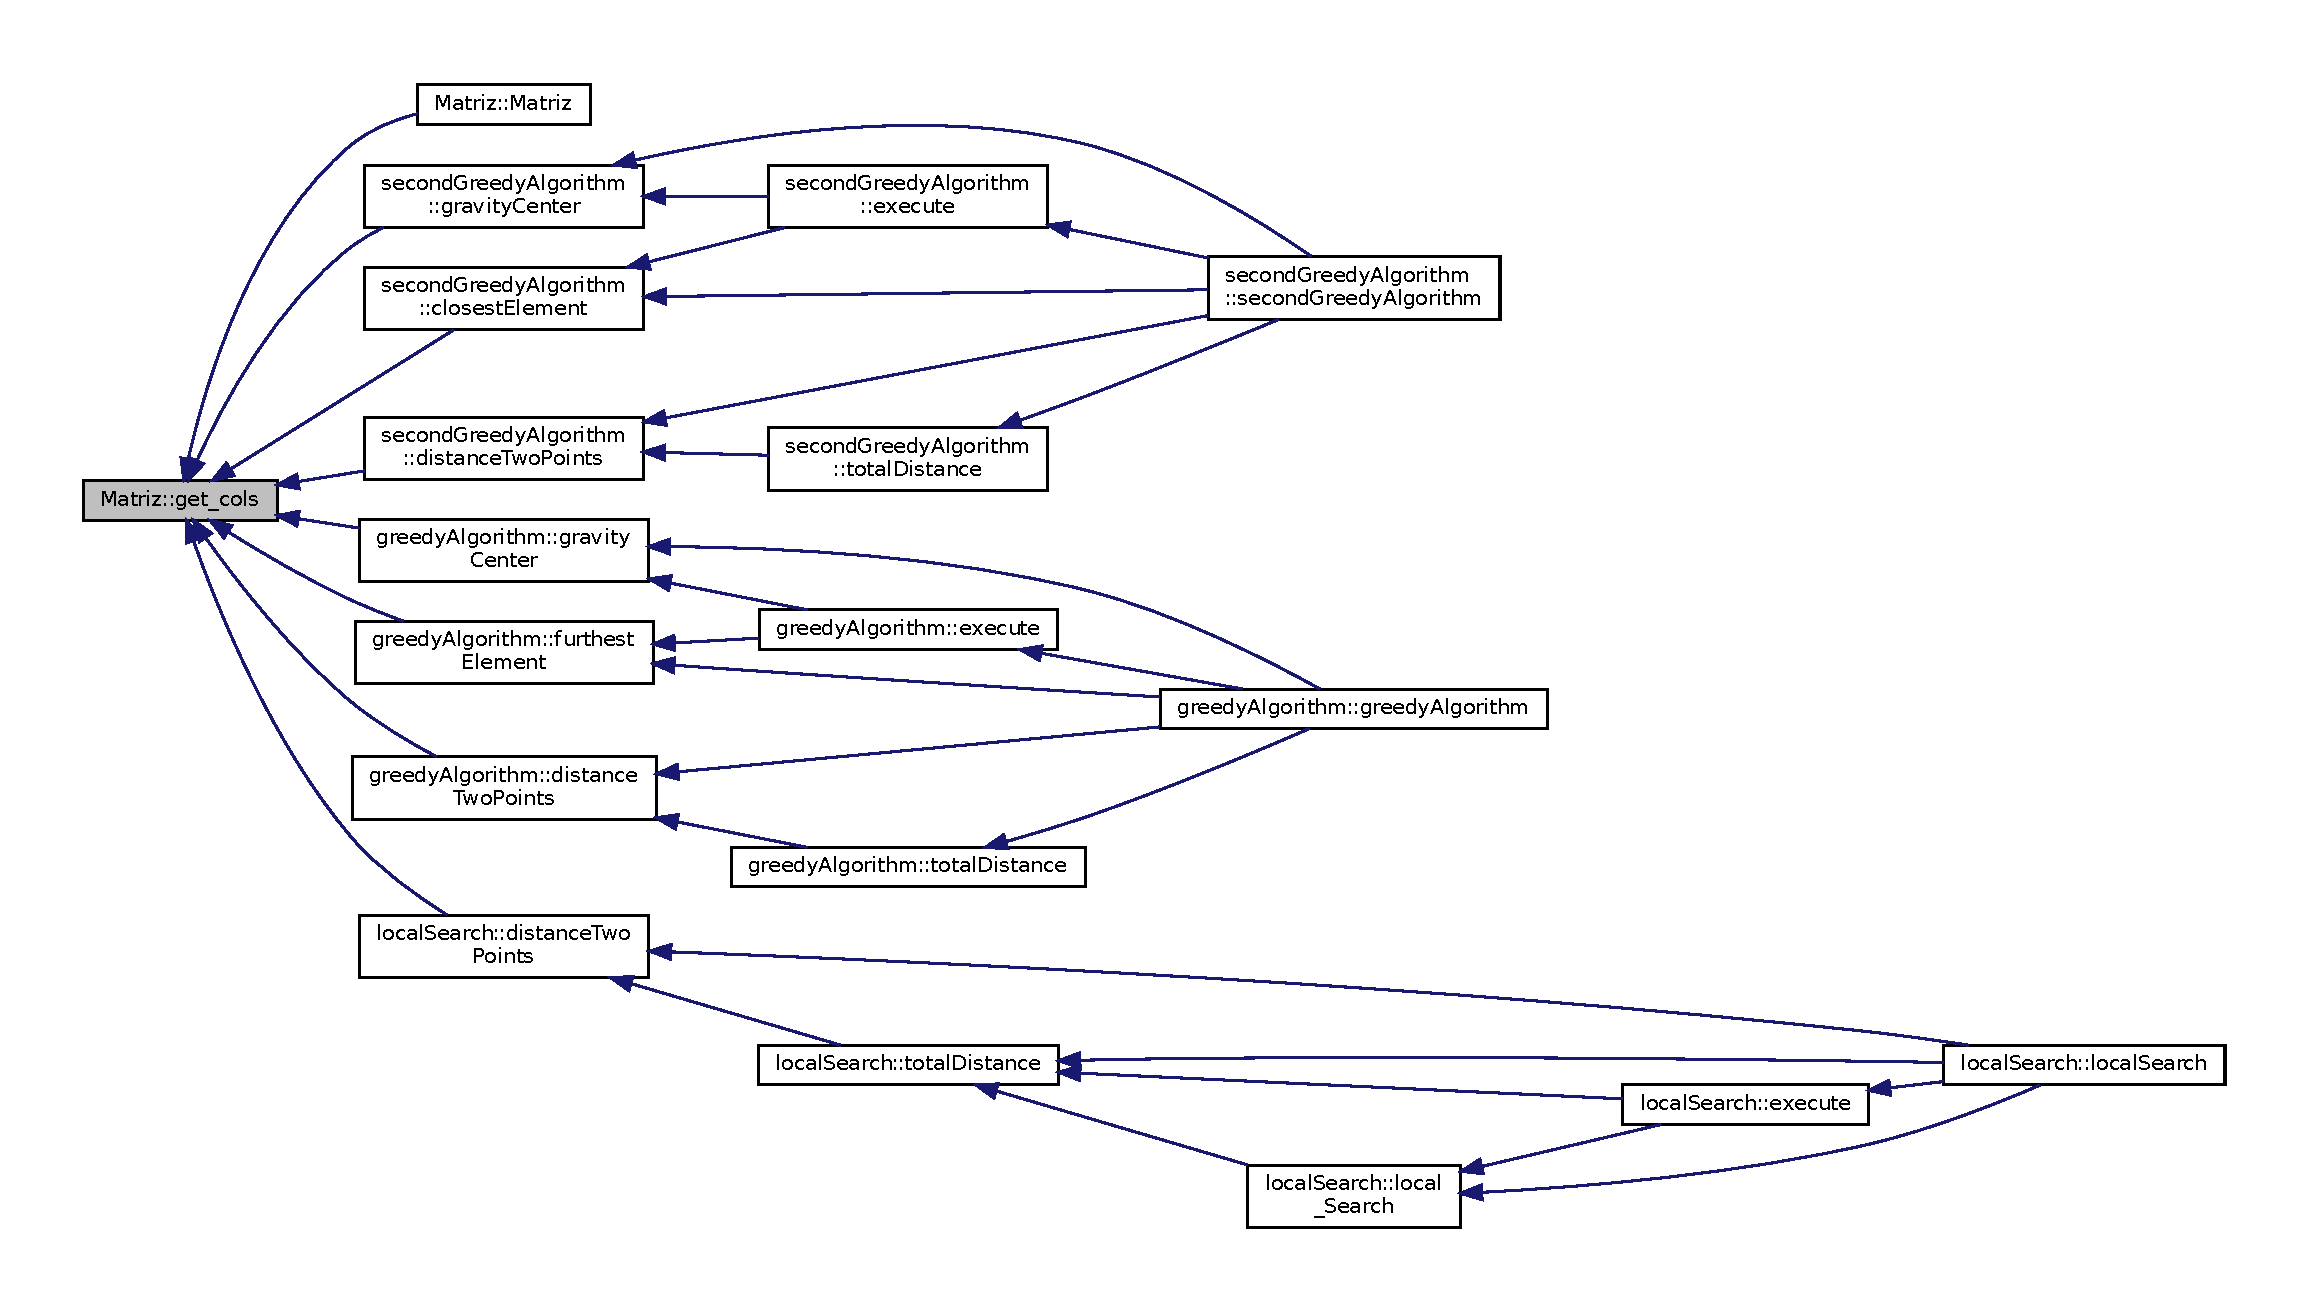
\includegraphics[width=350pt]{classMatriz_ad6915f9b31f93230a3ce05d01d23a47b_icgraph}
\end{center}
\end{figure}
\mbox{\Hypertarget{classMatriz_aaf1b9c3af2d3b269cc0a2dda08aebd61}\label{classMatriz_aaf1b9c3af2d3b269cc0a2dda08aebd61}} 
\index{Matriz@{Matriz}!get\+\_\+position@{get\+\_\+position}}
\index{get\+\_\+position@{get\+\_\+position}!Matriz@{Matriz}}
\subsubsection{\texorpdfstring{get\+\_\+position()}{get\_position()}}
{\footnotesize\ttfamily float Matriz\+::get\+\_\+position (\begin{DoxyParamCaption}\item[{int}]{row,  }\item[{int}]{col }\end{DoxyParamCaption})}



Get the position object. 


\begin{DoxyParams}{Parameters}
{\em row} & \\
\hline
{\em col} & \\
\hline
\end{DoxyParams}
\begin{DoxyReturn}{Returns}
float 
\end{DoxyReturn}

\begin{DoxyCode}
28 \{
29   \textcolor{keywordflow}{return} matrix[row][col];
30 \}
\end{DoxyCode}
Here is the caller graph for this function\+:
\nopagebreak
\begin{figure}[H]
\begin{center}
\leavevmode
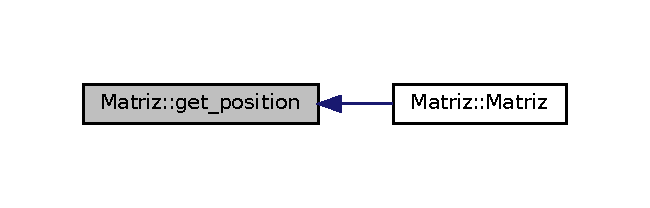
\includegraphics[width=312pt]{classMatriz_aaf1b9c3af2d3b269cc0a2dda08aebd61_icgraph}
\end{center}
\end{figure}
\mbox{\Hypertarget{classMatriz_a6b18342f8c083baece693ff41185a206}\label{classMatriz_a6b18342f8c083baece693ff41185a206}} 
\index{Matriz@{Matriz}!get\+\_\+rows@{get\+\_\+rows}}
\index{get\+\_\+rows@{get\+\_\+rows}!Matriz@{Matriz}}
\subsubsection{\texorpdfstring{get\+\_\+rows()}{get\_rows()}}
{\footnotesize\ttfamily int Matriz\+::get\+\_\+rows (\begin{DoxyParamCaption}{ }\end{DoxyParamCaption})}



Get the rows object. 

\begin{DoxyReturn}{Returns}
float 
\end{DoxyReturn}

\begin{DoxyCode}
13 \{
14   \textcolor{keywordflow}{return} matrix.size();
15 \}
\end{DoxyCode}
Here is the caller graph for this function\+:
\nopagebreak
\begin{figure}[H]
\begin{center}
\leavevmode
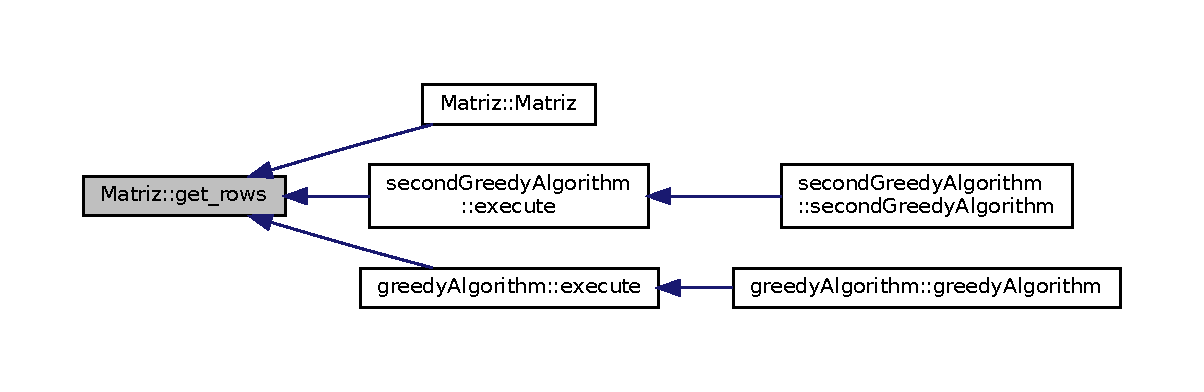
\includegraphics[width=350pt]{classMatriz_a6b18342f8c083baece693ff41185a206_icgraph}
\end{center}
\end{figure}
\mbox{\Hypertarget{classMatriz_a5516a9b9524e4604d4b3040628be50e9}\label{classMatriz_a5516a9b9524e4604d4b3040628be50e9}} 
\index{Matriz@{Matriz}!operator\mbox{[}\mbox{]}@{operator[]}}
\index{operator\mbox{[}\mbox{]}@{operator[]}!Matriz@{Matriz}}
\subsubsection{\texorpdfstring{operator[]()}{operator[]()}}
{\footnotesize\ttfamily std\+::vector$<$ float $>$ \& Matriz\+::operator\mbox{[}$\,$\mbox{]} (\begin{DoxyParamCaption}\item[{int}]{index }\end{DoxyParamCaption})}



Operator \mbox{[}\mbox{]} overload. 


\begin{DoxyParams}{Parameters}
{\em index} & \\
\hline
\end{DoxyParams}
\begin{DoxyReturn}{Returns}
std\+::vector$<$float$>$\& 
\end{DoxyReturn}

\begin{DoxyCode}
45 \{
46   \textcolor{keywordflow}{if} (index >= matrix.size())
47   \{
48     std::cerr << \textcolor{stringliteral}{"Index fuera de rango"} << std::endl;
49     std::exit(0);
50   \}
51   \textcolor{keywordflow}{else}
52   \{
53     \textcolor{keywordflow}{return} matrix[index];
54   \}
55 \}
\end{DoxyCode}
Here is the caller graph for this function\+:
\nopagebreak
\begin{figure}[H]
\begin{center}
\leavevmode
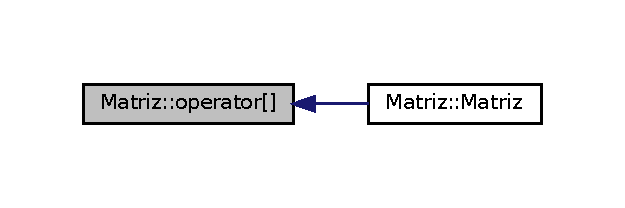
\includegraphics[width=300pt]{classMatriz_a5516a9b9524e4604d4b3040628be50e9_icgraph}
\end{center}
\end{figure}
\mbox{\Hypertarget{classMatriz_aa929f933e9088dc0efecaa9a46d555d9}\label{classMatriz_aa929f933e9088dc0efecaa9a46d555d9}} 
\index{Matriz@{Matriz}!resize\+Matrix@{resize\+Matrix}}
\index{resize\+Matrix@{resize\+Matrix}!Matriz@{Matriz}}
\subsubsection{\texorpdfstring{resize\+Matrix()}{resizeMatrix()}}
{\footnotesize\ttfamily void Matriz\+::resize\+Matrix (\begin{DoxyParamCaption}\item[{int}]{rows,  }\item[{int}]{cols }\end{DoxyParamCaption})}



Change the matrix\textquotesingle{}s dimensions. 


\begin{DoxyParams}{Parameters}
{\em rows} & \\
\hline
{\em cols} & \\
\hline
\end{DoxyParams}

\begin{DoxyCode}
4 \{
5   \textcolor{keywordflow}{for} (\textcolor{keywordtype}{int} i = 0; i < matrix.size(); i++)
6   \{
7     matrix[i].resize(cols);
8   \}
9   matrix.resize(rows, std::vector<float>(cols));
10 \}
\end{DoxyCode}
Here is the caller graph for this function\+:
\nopagebreak
\begin{figure}[H]
\begin{center}
\leavevmode
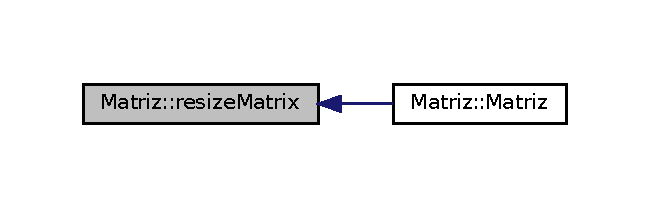
\includegraphics[width=312pt]{classMatriz_aa929f933e9088dc0efecaa9a46d555d9_icgraph}
\end{center}
\end{figure}
\mbox{\Hypertarget{classMatriz_a3641ea6e8f91cffd9073c22a71082cf8}\label{classMatriz_a3641ea6e8f91cffd9073c22a71082cf8}} 
\index{Matriz@{Matriz}!set\+\_\+position@{set\+\_\+position}}
\index{set\+\_\+position@{set\+\_\+position}!Matriz@{Matriz}}
\subsubsection{\texorpdfstring{set\+\_\+position()}{set\_position()}}
{\footnotesize\ttfamily void Matriz\+::set\+\_\+position (\begin{DoxyParamCaption}\item[{int}]{row,  }\item[{int}]{col,  }\item[{float}]{value }\end{DoxyParamCaption})}



Set the position object. 


\begin{DoxyParams}{Parameters}
{\em row} & \\
\hline
{\em col} & \\
\hline
{\em value} & \\
\hline
\end{DoxyParams}

\begin{DoxyCode}
23 \{
24   matrix[row][col] = value;
25 \}
\end{DoxyCode}
Here is the caller graph for this function\+:
\nopagebreak
\begin{figure}[H]
\begin{center}
\leavevmode
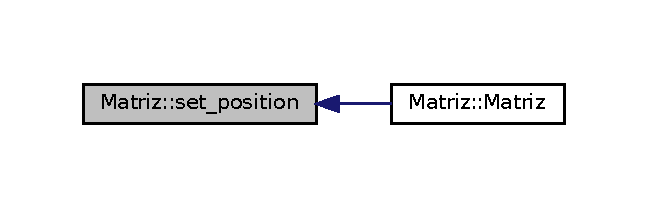
\includegraphics[width=311pt]{classMatriz_a3641ea6e8f91cffd9073c22a71082cf8_icgraph}
\end{center}
\end{figure}


The documentation for this class was generated from the following files\+:\begin{DoxyCompactItemize}
\item 
include/Matrix.\+hpp\item 
src/Matrix.\+cpp\end{DoxyCompactItemize}

\hypertarget{classsecondGreedyAlgorithm}{}\section{second\+Greedy\+Algorithm Class Reference}
\label{classsecondGreedyAlgorithm}\index{second\+Greedy\+Algorithm@{second\+Greedy\+Algorithm}}


Another implementation of the greedy algorithm to solve Maximum diversity problem.  




{\ttfamily \#include $<$2nd\+Greedy\+Algorithm.\+hpp$>$}



Inheritance diagram for second\+Greedy\+Algorithm\+:
\nopagebreak
\begin{figure}[H]
\begin{center}
\leavevmode
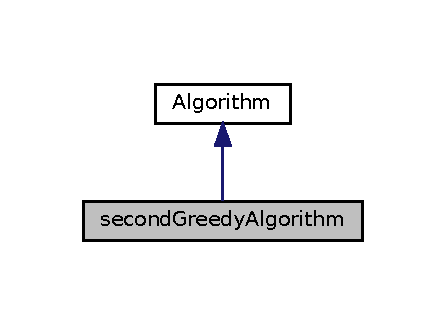
\includegraphics[width=214pt]{classsecondGreedyAlgorithm__inherit__graph}
\end{center}
\end{figure}


Collaboration diagram for second\+Greedy\+Algorithm\+:
\nopagebreak
\begin{figure}[H]
\begin{center}
\leavevmode
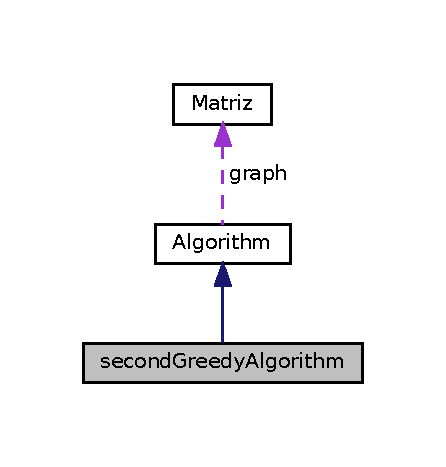
\includegraphics[width=214pt]{classsecondGreedyAlgorithm__coll__graph}
\end{center}
\end{figure}
\subsection*{Public Member Functions}
\begin{DoxyCompactItemize}
\item 
\hyperlink{classsecondGreedyAlgorithm_acbb57b3cc5b088ee401be24841e10eef}{second\+Greedy\+Algorithm} (std\+::string filename, int sol)
\begin{DoxyCompactList}\small\item\em Construct a new \hyperlink{classsecondGreedyAlgorithm}{second\+Greedy\+Algorithm} object. \end{DoxyCompactList}\item 
std\+::vector$<$ int $>$ \hyperlink{classsecondGreedyAlgorithm_a119a730116003d00438179ccf4e2cafd}{execute} ()
\begin{DoxyCompactList}\small\item\em Method that executes the algorithm. \end{DoxyCompactList}\item 
std\+::vector$<$ float $>$ \hyperlink{classsecondGreedyAlgorithm_a95e094bd3f2ee22127eaaf734c2cee8a}{gravity\+Center} (std\+::vector$<$ int $>$)
\begin{DoxyCompactList}\small\item\em Method that calculates the gravity center. \end{DoxyCompactList}\item 
int \hyperlink{classsecondGreedyAlgorithm_ad34d30fcba1f3d71dc67ea6b12d5d0b8}{closest\+Element} (std\+::vector$<$ int $>$, std\+::vector$<$ float $>$)
\begin{DoxyCompactList}\small\item\em Returns the index of the closest element to the center. \end{DoxyCompactList}\item 
float \hyperlink{classsecondGreedyAlgorithm_a21a936acf628b02184e745faf918618a}{total\+Distance} (std\+::vector$<$ int $>$)
\begin{DoxyCompactList}\small\item\em Method that computes the total distance given a solution. \end{DoxyCompactList}\item 
float \hyperlink{classsecondGreedyAlgorithm_a72574b0ef83083f7994af0eb4007cf39}{distance\+Two\+Points} (int, int)
\begin{DoxyCompactList}\small\item\em Calculates the distance between two points. \end{DoxyCompactList}\end{DoxyCompactItemize}
\subsection*{Additional Inherited Members}


\subsection{Detailed Description}
Another implementation of the greedy algorithm to solve Maximum diversity problem. 

\subsection{Constructor \& Destructor Documentation}
\mbox{\Hypertarget{classsecondGreedyAlgorithm_acbb57b3cc5b088ee401be24841e10eef}\label{classsecondGreedyAlgorithm_acbb57b3cc5b088ee401be24841e10eef}} 
\index{second\+Greedy\+Algorithm@{second\+Greedy\+Algorithm}!second\+Greedy\+Algorithm@{second\+Greedy\+Algorithm}}
\index{second\+Greedy\+Algorithm@{second\+Greedy\+Algorithm}!second\+Greedy\+Algorithm@{second\+Greedy\+Algorithm}}
\subsubsection{\texorpdfstring{second\+Greedy\+Algorithm()}{secondGreedyAlgorithm()}}
{\footnotesize\ttfamily second\+Greedy\+Algorithm\+::second\+Greedy\+Algorithm (\begin{DoxyParamCaption}\item[{std\+::string}]{filename,  }\item[{int}]{sol }\end{DoxyParamCaption})\hspace{0.3cm}{\ttfamily [inline]}}



Construct a new \hyperlink{classsecondGreedyAlgorithm}{second\+Greedy\+Algorithm} object. 


\begin{DoxyParams}{Parameters}
{\em filename} & \\
\hline
\end{DoxyParams}

\begin{DoxyCode}
31 : \hyperlink{classAlgorithm_a3c199c8528aae86f06ac515d5102fa09}{Algorithm}(filename, sol) \{\}
\end{DoxyCode}
Here is the call graph for this function\+:
\nopagebreak
\begin{figure}[H]
\begin{center}
\leavevmode
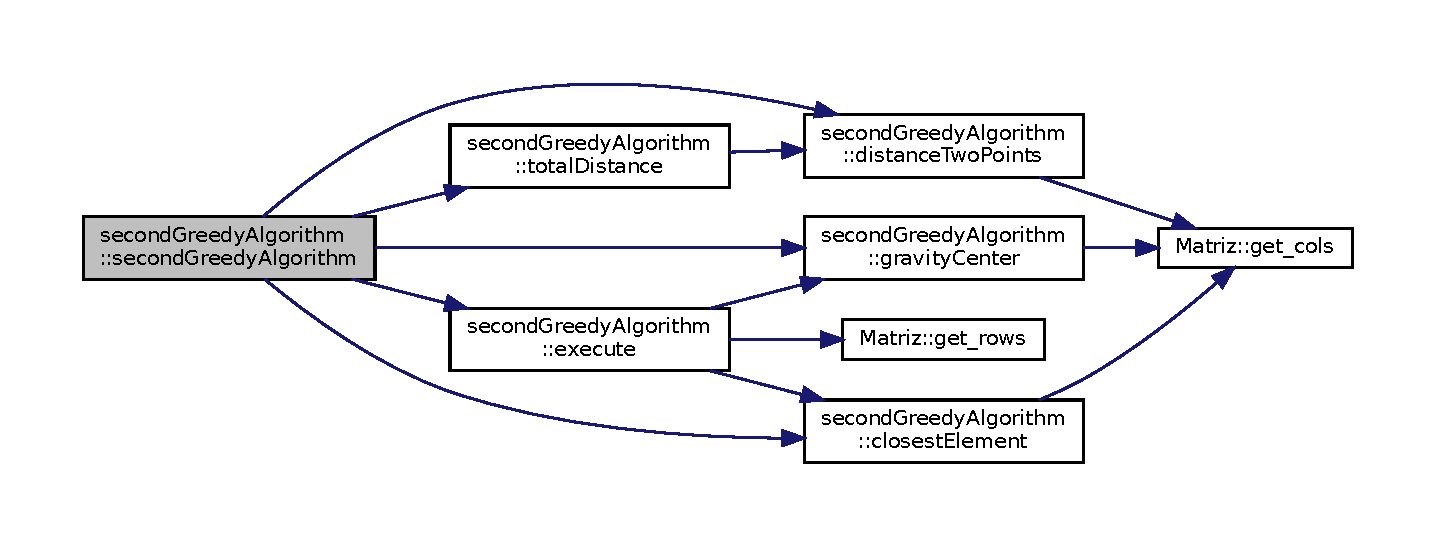
\includegraphics[width=350pt]{classsecondGreedyAlgorithm_acbb57b3cc5b088ee401be24841e10eef_cgraph}
\end{center}
\end{figure}


\subsection{Member Function Documentation}
\mbox{\Hypertarget{classsecondGreedyAlgorithm_ad34d30fcba1f3d71dc67ea6b12d5d0b8}\label{classsecondGreedyAlgorithm_ad34d30fcba1f3d71dc67ea6b12d5d0b8}} 
\index{second\+Greedy\+Algorithm@{second\+Greedy\+Algorithm}!closest\+Element@{closest\+Element}}
\index{closest\+Element@{closest\+Element}!second\+Greedy\+Algorithm@{second\+Greedy\+Algorithm}}
\subsubsection{\texorpdfstring{closest\+Element()}{closestElement()}}
{\footnotesize\ttfamily int second\+Greedy\+Algorithm\+::closest\+Element (\begin{DoxyParamCaption}\item[{std\+::vector$<$ int $>$}]{Elem,  }\item[{std\+::vector$<$ float $>$}]{SC }\end{DoxyParamCaption})}



Returns the index of the closest element to the center. 

\begin{DoxyReturn}{Returns}
int 
\end{DoxyReturn}

\begin{DoxyCode}
31                                                                                   \{
32   \textcolor{keywordtype}{float} distance = 1000000;
33   \textcolor{keywordtype}{int} solution = 0;
34   std::vector<int> repetidos;
35   \textcolor{keywordflow}{for}(\textcolor{keywordtype}{int} i = 0; i < Elem.size(); i++) \{
36     \textcolor{keywordtype}{float} sum = 0;
37     \textcolor{keywordflow}{for}(\textcolor{keywordtype}{int} j = 0; j < graph.\hyperlink{classMatriz_ad6915f9b31f93230a3ce05d01d23a47b}{get\_cols}(); j++) \{
38       sum += pow(SC[j] - graph[Elem[i]][j], 2);
39     \}
40     sum = sqrt(sum);
41     \textcolor{keywordflow}{if}(sum < distance) \{
42       distance = sum;
43       solution = Elem[i];
44       repetidos.clear();
45       repetidos.push\_back(Elem[i]);
46     \} \textcolor{keywordflow}{else} \textcolor{keywordflow}{if}(sum == distance) \{
47       repetidos.push\_back(Elem[i]);
48     \}
49   \}
50   \textcolor{keywordflow}{if}(repetidos.size() > 1) \{
51     \textcolor{keywordtype}{int} index = std::rand() % repetidos.size();
52     \textcolor{keywordflow}{return} repetidos[index];
53   \}
54   \textcolor{keywordflow}{return} solution;
55 \}
\end{DoxyCode}
Here is the call graph for this function\+:
\nopagebreak
\begin{figure}[H]
\begin{center}
\leavevmode
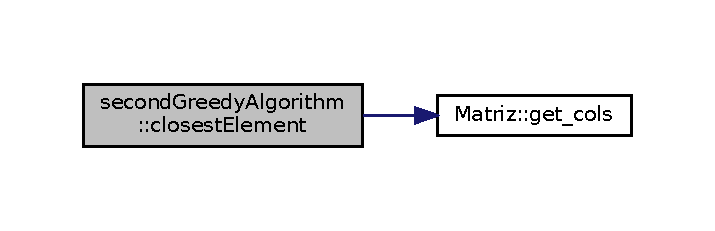
\includegraphics[width=343pt]{classsecondGreedyAlgorithm_ad34d30fcba1f3d71dc67ea6b12d5d0b8_cgraph}
\end{center}
\end{figure}
Here is the caller graph for this function\+:
\nopagebreak
\begin{figure}[H]
\begin{center}
\leavevmode
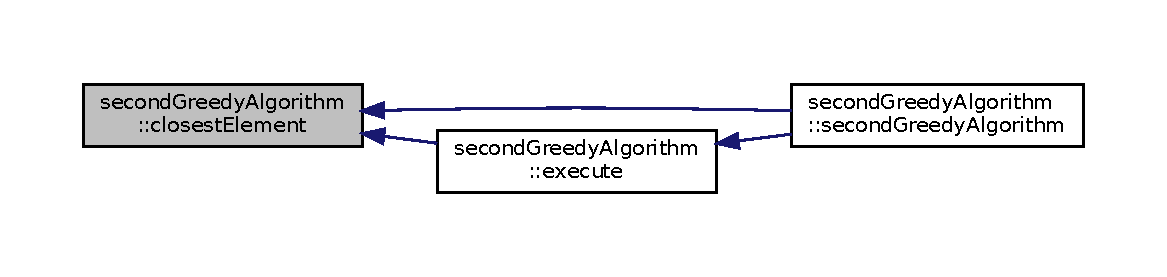
\includegraphics[width=350pt]{classsecondGreedyAlgorithm_ad34d30fcba1f3d71dc67ea6b12d5d0b8_icgraph}
\end{center}
\end{figure}
\mbox{\Hypertarget{classsecondGreedyAlgorithm_a72574b0ef83083f7994af0eb4007cf39}\label{classsecondGreedyAlgorithm_a72574b0ef83083f7994af0eb4007cf39}} 
\index{second\+Greedy\+Algorithm@{second\+Greedy\+Algorithm}!distance\+Two\+Points@{distance\+Two\+Points}}
\index{distance\+Two\+Points@{distance\+Two\+Points}!second\+Greedy\+Algorithm@{second\+Greedy\+Algorithm}}
\subsubsection{\texorpdfstring{distance\+Two\+Points()}{distanceTwoPoints()}}
{\footnotesize\ttfamily float second\+Greedy\+Algorithm\+::distance\+Two\+Points (\begin{DoxyParamCaption}\item[{int}]{point1,  }\item[{int}]{point2 }\end{DoxyParamCaption})}



Calculates the distance between two points. 

\begin{DoxyReturn}{Returns}
float 
\end{DoxyReturn}

\begin{DoxyCode}
67                                                                      \{
68   \textcolor{keywordtype}{float} sum = 0; 
69   \textcolor{keywordflow}{for}(\textcolor{keywordtype}{int} j = 0; j < graph.\hyperlink{classMatriz_ad6915f9b31f93230a3ce05d01d23a47b}{get\_cols}(); j++) \{
70     sum += pow(graph[point1][j] - graph[point2][j], 2);
71   \}
72   sum = sqrt(sum);
73   \textcolor{keywordflow}{return} sum;
74 \}
\end{DoxyCode}
Here is the call graph for this function\+:
\nopagebreak
\begin{figure}[H]
\begin{center}
\leavevmode
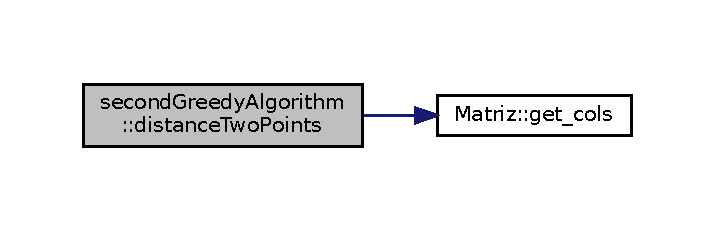
\includegraphics[width=343pt]{classsecondGreedyAlgorithm_a72574b0ef83083f7994af0eb4007cf39_cgraph}
\end{center}
\end{figure}
Here is the caller graph for this function\+:
\nopagebreak
\begin{figure}[H]
\begin{center}
\leavevmode
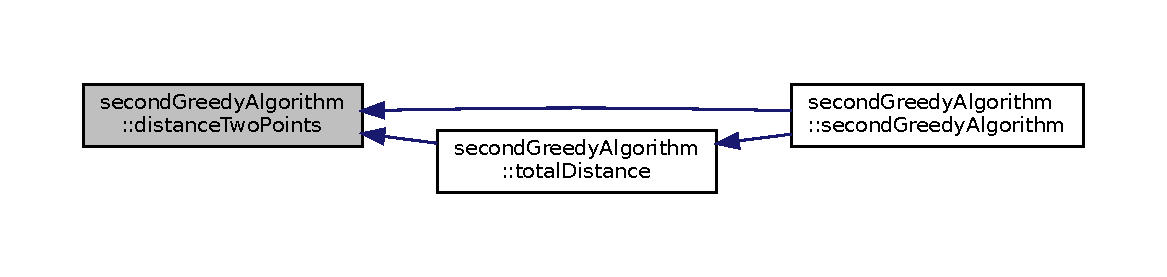
\includegraphics[width=350pt]{classsecondGreedyAlgorithm_a72574b0ef83083f7994af0eb4007cf39_icgraph}
\end{center}
\end{figure}
\mbox{\Hypertarget{classsecondGreedyAlgorithm_a119a730116003d00438179ccf4e2cafd}\label{classsecondGreedyAlgorithm_a119a730116003d00438179ccf4e2cafd}} 
\index{second\+Greedy\+Algorithm@{second\+Greedy\+Algorithm}!execute@{execute}}
\index{execute@{execute}!second\+Greedy\+Algorithm@{second\+Greedy\+Algorithm}}
\subsubsection{\texorpdfstring{execute()}{execute()}}
{\footnotesize\ttfamily std\+::vector$<$ int $>$ second\+Greedy\+Algorithm\+::execute (\begin{DoxyParamCaption}{ }\end{DoxyParamCaption})\hspace{0.3cm}{\ttfamily [virtual]}}



Method that executes the algorithm. 

\begin{DoxyReturn}{Returns}
std\+::vector$<$float$>$ 
\end{DoxyReturn}


Implements \hyperlink{classAlgorithm_af6ea9eb9a6dbd41896e3fd7dabac096b}{Algorithm}.


\begin{DoxyCode}
4 \{
5   std::vector<int> solution;
6   \textcolor{keywordflow}{for} (\textcolor{keywordtype}{int} i = 0; i < graph.\hyperlink{classMatriz_a6b18342f8c083baece693ff41185a206}{get\_rows}(); i++)
7   \{
8     solution.push\_back(i);
9   \}
10   std::vector<float> SC = \hyperlink{classsecondGreedyAlgorithm_a95e094bd3f2ee22127eaaf734c2cee8a}{gravityCenter}(solution);
11   \textcolor{keywordflow}{while}(solution.size() != solutionSize) \{
12     \textcolor{keywordtype}{int} close = \hyperlink{classsecondGreedyAlgorithm_ad34d30fcba1f3d71dc67ea6b12d5d0b8}{closestElement}(solution, SC);
13     solution.erase(std::find(solution.begin(), solution.end(), close));
14     SC = \hyperlink{classsecondGreedyAlgorithm_a95e094bd3f2ee22127eaaf734c2cee8a}{gravityCenter}(solution);
15   \}
16   \textcolor{keywordflow}{return} solution;
17 \}
\end{DoxyCode}
Here is the call graph for this function\+:
\nopagebreak
\begin{figure}[H]
\begin{center}
\leavevmode
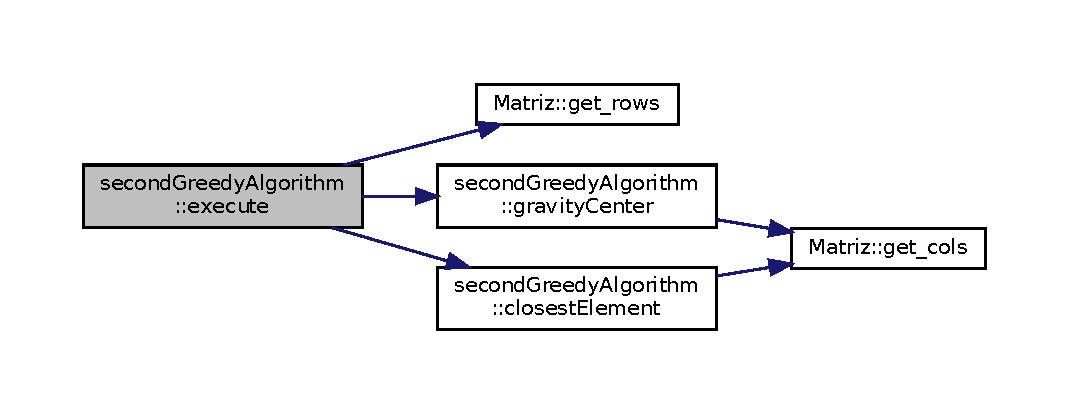
\includegraphics[width=350pt]{classsecondGreedyAlgorithm_a119a730116003d00438179ccf4e2cafd_cgraph}
\end{center}
\end{figure}
Here is the caller graph for this function\+:
\nopagebreak
\begin{figure}[H]
\begin{center}
\leavevmode
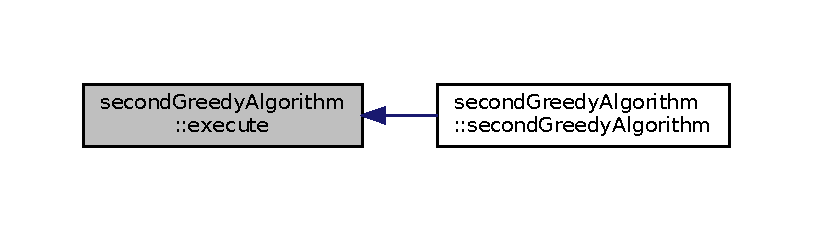
\includegraphics[width=350pt]{classsecondGreedyAlgorithm_a119a730116003d00438179ccf4e2cafd_icgraph}
\end{center}
\end{figure}
\mbox{\Hypertarget{classsecondGreedyAlgorithm_a95e094bd3f2ee22127eaaf734c2cee8a}\label{classsecondGreedyAlgorithm_a95e094bd3f2ee22127eaaf734c2cee8a}} 
\index{second\+Greedy\+Algorithm@{second\+Greedy\+Algorithm}!gravity\+Center@{gravity\+Center}}
\index{gravity\+Center@{gravity\+Center}!second\+Greedy\+Algorithm@{second\+Greedy\+Algorithm}}
\subsubsection{\texorpdfstring{gravity\+Center()}{gravityCenter()}}
{\footnotesize\ttfamily std\+::vector$<$ float $>$ second\+Greedy\+Algorithm\+::gravity\+Center (\begin{DoxyParamCaption}\item[{std\+::vector$<$ int $>$}]{Elem }\end{DoxyParamCaption})}



Method that calculates the gravity center. 

\begin{DoxyReturn}{Returns}
std\+::vector$<$float$>$ 
\end{DoxyReturn}

\begin{DoxyCode}
19                                                                          \{
20   std::vector<float> solution;
21   \textcolor{keywordflow}{for}(\textcolor{keywordtype}{int} i = 0; i < graph.\hyperlink{classMatriz_ad6915f9b31f93230a3ce05d01d23a47b}{get\_cols}(); i++) \{
22     \textcolor{keywordtype}{float} sum = 0;
23     \textcolor{keywordflow}{for}(\textcolor{keywordtype}{int} j = 0; j < Elem.size(); j++) \{      
24       sum += graph[Elem[j]][i]; 
25     \}
26     solution.push\_back(sum / Elem.size());
27   \}
28   \textcolor{keywordflow}{return} solution;
29 \}
\end{DoxyCode}
Here is the call graph for this function\+:
\nopagebreak
\begin{figure}[H]
\begin{center}
\leavevmode
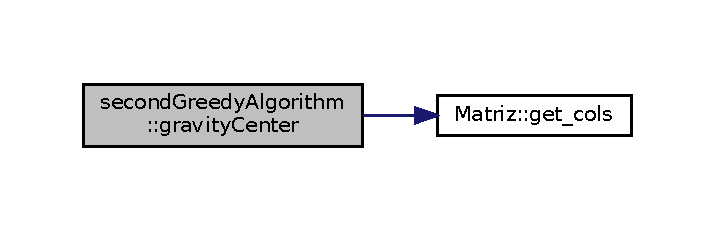
\includegraphics[width=343pt]{classsecondGreedyAlgorithm_a95e094bd3f2ee22127eaaf734c2cee8a_cgraph}
\end{center}
\end{figure}
Here is the caller graph for this function\+:
\nopagebreak
\begin{figure}[H]
\begin{center}
\leavevmode
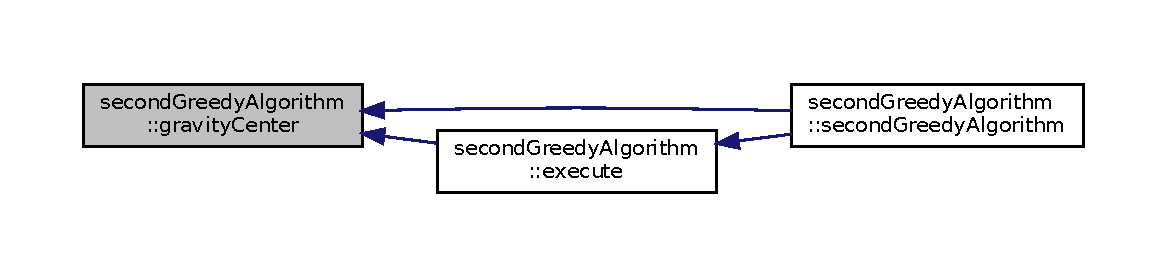
\includegraphics[width=350pt]{classsecondGreedyAlgorithm_a95e094bd3f2ee22127eaaf734c2cee8a_icgraph}
\end{center}
\end{figure}
\mbox{\Hypertarget{classsecondGreedyAlgorithm_a21a936acf628b02184e745faf918618a}\label{classsecondGreedyAlgorithm_a21a936acf628b02184e745faf918618a}} 
\index{second\+Greedy\+Algorithm@{second\+Greedy\+Algorithm}!total\+Distance@{total\+Distance}}
\index{total\+Distance@{total\+Distance}!second\+Greedy\+Algorithm@{second\+Greedy\+Algorithm}}
\subsubsection{\texorpdfstring{total\+Distance()}{totalDistance()}}
{\footnotesize\ttfamily float second\+Greedy\+Algorithm\+::total\+Distance (\begin{DoxyParamCaption}\item[{std\+::vector$<$ int $>$}]{solution }\end{DoxyParamCaption})}



Method that computes the total distance given a solution. 

\begin{DoxyReturn}{Returns}
float 
\end{DoxyReturn}

\begin{DoxyCode}
57                                                                   \{
58   \textcolor{keywordtype}{float} sum = 0;
59   \textcolor{keywordflow}{for}(\textcolor{keywordtype}{int} i = 0; i < solution.size(); i++) \{
60     \textcolor{keywordflow}{for}(\textcolor{keywordtype}{int} j = i + 1; j < solution.size(); j++) \{
61       sum += \hyperlink{classsecondGreedyAlgorithm_a72574b0ef83083f7994af0eb4007cf39}{distanceTwoPoints}(solution[i], solution[j]);
62     \}
63   \}
64   \textcolor{keywordflow}{return} sum;
65 \}
\end{DoxyCode}
Here is the call graph for this function\+:
\nopagebreak
\begin{figure}[H]
\begin{center}
\leavevmode
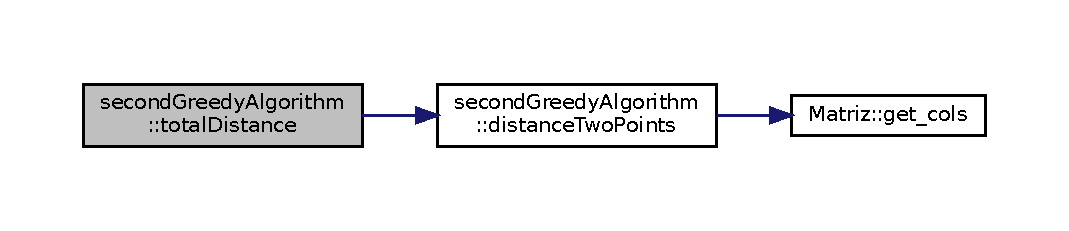
\includegraphics[width=350pt]{classsecondGreedyAlgorithm_a21a936acf628b02184e745faf918618a_cgraph}
\end{center}
\end{figure}
Here is the caller graph for this function\+:
\nopagebreak
\begin{figure}[H]
\begin{center}
\leavevmode
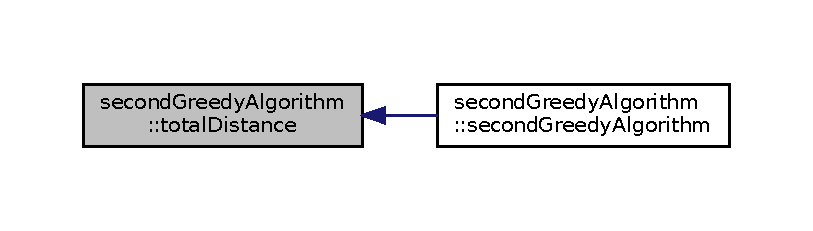
\includegraphics[width=350pt]{classsecondGreedyAlgorithm_a21a936acf628b02184e745faf918618a_icgraph}
\end{center}
\end{figure}


The documentation for this class was generated from the following files\+:\begin{DoxyCompactItemize}
\item 
include/\hyperlink{2ndGreedyAlgorithm_8hpp}{2nd\+Greedy\+Algorithm.\+hpp}\item 
src/2nd\+Greedy\+Algorithm.\+cpp\end{DoxyCompactItemize}

\chapter{File Documentation}
\hypertarget{2ndGreedyAlgorithm_8hpp}{}\section{include/2nd\+Greedy\+Algorithm.hpp File Reference}
\label{2ndGreedyAlgorithm_8hpp}\index{include/2nd\+Greedy\+Algorithm.\+hpp@{include/2nd\+Greedy\+Algorithm.\+hpp}}


Fichero que contiene la implementación del algoritmo greedy de forma destructiva.  


{\ttfamily \#include \char`\"{}Matrix.\+hpp\char`\"{}}\newline
{\ttfamily \#include \char`\"{}algorithm.\+hpp\char`\"{}}\newline
{\ttfamily \#include \char`\"{}math.\+h\char`\"{}}\newline
Include dependency graph for 2nd\+Greedy\+Algorithm.hpp\+:
\nopagebreak
\begin{figure}[H]
\begin{center}
\leavevmode
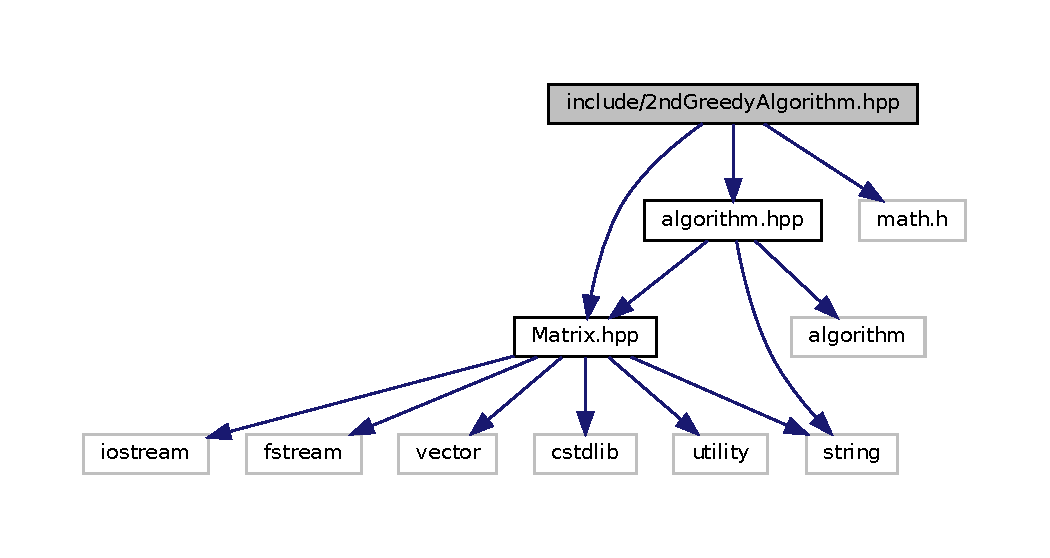
\includegraphics[width=350pt]{2ndGreedyAlgorithm_8hpp__incl}
\end{center}
\end{figure}
\subsection*{Classes}
\begin{DoxyCompactItemize}
\item 
class \hyperlink{classsecondGreedyAlgorithm}{second\+Greedy\+Algorithm}
\begin{DoxyCompactList}\small\item\em Another implementation of the greedy algorithm to solve Maximum diversity problem. \end{DoxyCompactList}\end{DoxyCompactItemize}


\subsection{Detailed Description}
Fichero que contiene la implementación del algoritmo greedy de forma destructiva. 

\begin{DoxyAuthor}{Author}
Guillermo Hernández González 
\end{DoxyAuthor}
\begin{DoxyVersion}{Version}
1.\+0 
\end{DoxyVersion}
\begin{DoxyDate}{Date}
2020-\/05-\/18
\end{DoxyDate}
\begin{DoxyCopyright}{Copyright}
Copyright (c) 2020 
\end{DoxyCopyright}

\hypertarget{algorithm_8hpp}{}\section{include/algorithm.hpp File Reference}
\label{algorithm_8hpp}\index{include/algorithm.\+hpp@{include/algorithm.\+hpp}}


Fichero que contiene la clase \hyperlink{classAlgorithm}{Algorithm} que servirá como clase base para la implementación de los otros algoritmos.  


{\ttfamily \#include $<$string$>$}\newline
{\ttfamily \#include $<$algorithm$>$}\newline
{\ttfamily \#include \char`\"{}Matrix.\+hpp\char`\"{}}\newline
Include dependency graph for algorithm.\+hpp\+:
\nopagebreak
\begin{figure}[H]
\begin{center}
\leavevmode
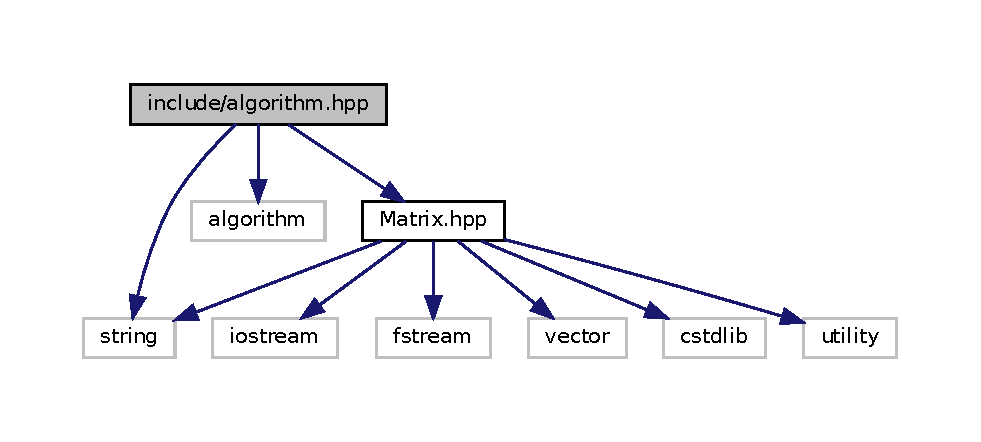
\includegraphics[width=350pt]{algorithm_8hpp__incl}
\end{center}
\end{figure}
This graph shows which files directly or indirectly include this file\+:
\nopagebreak
\begin{figure}[H]
\begin{center}
\leavevmode
\includegraphics[width=350pt]{algorithm_8hpp__dep__incl}
\end{center}
\end{figure}
\subsection*{Classes}
\begin{DoxyCompactItemize}
\item 
class \hyperlink{classAlgorithm}{Algorithm}
\begin{DoxyCompactList}\small\item\em virtual algorithm class used to solve the maxmean problem \end{DoxyCompactList}\end{DoxyCompactItemize}


\subsection{Detailed Description}
Fichero que contiene la clase \hyperlink{classAlgorithm}{Algorithm} que servirá como clase base para la implementación de los otros algoritmos. 

\begin{DoxyAuthor}{Author}
Guillermo Hernández González 
\end{DoxyAuthor}
\begin{DoxyVersion}{Version}
1.\+0 
\end{DoxyVersion}
\begin{DoxyDate}{Date}
2020-\/04-\/27
\end{DoxyDate}
\begin{DoxyCopyright}{Copyright}
Copyright (c) 2020 
\end{DoxyCopyright}

\hypertarget{greedyAlgorithm_8hpp}{}\section{include/greedy\+Algorithm.hpp File Reference}
\label{greedyAlgorithm_8hpp}\index{include/greedy\+Algorithm.\+hpp@{include/greedy\+Algorithm.\+hpp}}


Fichero que contiene la implementación del algoritmo greedy de forma constructiva.  


{\ttfamily \#include \char`\"{}Matrix.\+hpp\char`\"{}}\newline
{\ttfamily \#include \char`\"{}algorithm.\+hpp\char`\"{}}\newline
{\ttfamily \#include \char`\"{}math.\+h\char`\"{}}\newline
Include dependency graph for greedy\+Algorithm.\+hpp\+:
\nopagebreak
\begin{figure}[H]
\begin{center}
\leavevmode
\includegraphics[width=350pt]{greedyAlgorithm_8hpp__incl}
\end{center}
\end{figure}
\subsection*{Classes}
\begin{DoxyCompactItemize}
\item 
class \hyperlink{classgreedyAlgorithm}{greedy\+Algorithm}
\begin{DoxyCompactList}\small\item\em Implementation of the greedy algorithm to solve Maximum diversity problem. \end{DoxyCompactList}\end{DoxyCompactItemize}


\subsection{Detailed Description}
Fichero que contiene la implementación del algoritmo greedy de forma constructiva. 

\begin{DoxyAuthor}{Author}
Guillermo Hernández González 
\end{DoxyAuthor}
\begin{DoxyVersion}{Version}
1.\+0 
\end{DoxyVersion}
\begin{DoxyDate}{Date}
2020-\/05-\/18
\end{DoxyDate}
\begin{DoxyCopyright}{Copyright}
Copyright (c) 2020 
\end{DoxyCopyright}

\hypertarget{localSearch_8hpp}{}\section{include/local\+Search.hpp File Reference}
\label{localSearch_8hpp}\index{include/local\+Search.\+hpp@{include/local\+Search.\+hpp}}


Fichero que contiene la implementación de la búsqueda local.  


{\ttfamily \#include \char`\"{}Matrix.\+hpp\char`\"{}}\newline
{\ttfamily \#include \char`\"{}algorithm.\+hpp\char`\"{}}\newline
{\ttfamily \#include \char`\"{}math.\+h\char`\"{}}\newline
Include dependency graph for local\+Search.\+hpp\+:
\nopagebreak
\begin{figure}[H]
\begin{center}
\leavevmode
\includegraphics[width=350pt]{localSearch_8hpp__incl}
\end{center}
\end{figure}
\subsection*{Classes}
\begin{DoxyCompactItemize}
\item 
class \hyperlink{classlocalSearch}{local\+Search}
\begin{DoxyCompactList}\small\item\em Implementation of the Local Search algorithm. \end{DoxyCompactList}\end{DoxyCompactItemize}


\subsection{Detailed Description}
Fichero que contiene la implementación de la búsqueda local. 

\begin{DoxyAuthor}{Author}
Guillermo Hernández González 
\end{DoxyAuthor}
\begin{DoxyVersion}{Version}
1.\+0 
\end{DoxyVersion}
\begin{DoxyDate}{Date}
2020-\/05-\/18
\end{DoxyDate}
\begin{DoxyCopyright}{Copyright}
Copyright (c) 2020 
\end{DoxyCopyright}

%--- End generated contents ---

% Index
\backmatter
\newpage
\phantomsection
\clearemptydoublepage
\addcontentsline{toc}{chapter}{Index}
\printindex

\end{document}
